%DONE: Anonymise: remove reference to OMT paper.
%TODO: Improve grayscaling?
%DONE: Separate Appendix and Online Appendix files.
%DONE: Fix references to appendixes to follow the style of Table A.1, A.2 etc
%DONE: Compress Abstract to within 150 words.
%DONE: Create separate detailed title page with name and contact info.
%DONE: Provide a short list of appropriate reviewers. Jack Paine etc.

% {{{ Header
\documentclass[12pt]{article}
\usepackage{authblk}
\usepackage{booktabs}
\usepackage{caption}
%\usepackage{dcolumn}
\usepackage{fancyhdr}
\usepackage{graphicx}
\usepackage{hyperref}
\usepackage{import}
\usepackage[utf8]{inputenc}
\usepackage{longtable}
\usepackage{multicol}
\usepackage{natbib}
\usepackage{rotating}
\usepackage{setspace} \doublespacing
\usepackage{tabularx}

%\usepackage{mlmodern}
%\usepackage{ebgaramond}

% Setting color for hyperlinks
\hypersetup{
	colorlinks=true,
	citecolor=black,
	urlcolor=blue,
}

% Fix issue with links in references
\renewcommand{\harvardurl}{\textbf{URL:} \url}

% Changing the format of the affiliation 
\renewcommand\Affilfont{\itshape\small}

% Fixing separate page count for appendix
\newcounter{apppage}
\fancyhf{}% Clear fancy header/footer
\fancyfoot[C]{Page~\thepage~of~\pageref{lastpage}}
\pagestyle{plain}

% Front page
\title{After Forever: Pre-Colonial States and Civil Conflict}
\author{}
%\affil[$\dagger$]{Department of Sociology and Political Science, NTNU}

\date{}

\providecommand{\keywords}[1]
{
	\small	
	\textbf{\textit{Keywords---}} #1
}

\begin{document}

\maketitle

%}}}

\begin{abstract}

%[Alternative titles: "Distance does not make the heart grow fonder: Subtitle"
%"The Legacy: Subtitle"]

This paper argues that the historical presence of pre-colonial states can be
conflict inducing or reducing depending on the relationship between the
pre-colonial and post-independence states. To test this argument the paper
introduces new geospatial data that moves beyond the two dimensional
representation of state borders to provide a topographic measure of historical
state presence of 82 independent states in Africa in the 1800-1914 period. I
find that higher levels of pre-colonial state presence are conflict reducing in
areas surrounding modern capital cities. While in areas further away from the
post-independence capital, higher levels of pre-colonial statehood are found to
be conflict inducing. I argue that pre-colonial state legacies can provide
continuity of traditions and conflict reducing institutions. Nevertheless, in
more remote areas state legacies can also represent symbols of past independence
and leave behind regional elite networks who can violently resist the influence
of national governments.

\end{abstract}

\clearpage

Within the emerging literature on how independent pre-colonial African polities
have shaped post independence conflict, findings appear contradictory. Some
find a conflict inducing effect attributed to differences between ethnic groups with
and without histories of statehood \citep{Englebert2002, Paine2019}, others find
a conflict reducing effect from institutions generated by these states
\citep{Depetris-Chauvin2016, Wig2016}.

This paper addresses the apparent puzzle by arguing that the effect of
pre-colonial states on civil conflict, at the local level, is conditioned by the
relationship between the pre-colonial and post-independence states. On the one
hand, pre-colonial states can form the basis of the post-independence state. On
the other hand, pre-colonial states can form the basis of regional competitors
to the post-independence state. I argue that whether a pre-colonial state looks
more like the former than the latter can be proxied by the distance to the
post-independence capital. Close to capitals, high levels of pre-colonial state
presence reflect a degree of continuation of rule, providing legitimacy and
institutions that are peace inducing. Conversely, low levels of state presence
near the capital reflect a relative lack of foundation for the modern state.
Outside of capital areas the story is reversed. As African states gradually
expanded their reach into their own territories, they threatened the autonomy of
regional elites. When local elites stem from pre-colonial states they form more
cohesive and vertical structures, and can use powerful symbols of independence
to mobilize. The threat to autonomy triggers commitment problems. If regional
elites accept government demands they are no longer able to punish the
government if it later reneges on the deal.\footnote{Similar to the dynamic
between armed groups and the government.} Given that the capabilities of the
state (both militarily and in terms of gathering information) diminish over
distance, and the capabilities of pre-colonial state groups to organize, the
parties are evenly matched with limited information and commitment issues
present. In other words bargaining is likely to break down and be difficult to
reestablish.

Nigeria provides an illustrative example. Northern Nigeria is dominated by the
two former empires of the Sokoto Caliphate (and its twin state Adamawa) and
Borno (also referred to as Kanem-Borno), which form the basis of the
Muslim-North--Christian-South division of the country (see figure
\ref{nigeria}). The North has seen much civil violence in the post-cold war
period. Boko Haram, who has been responsible for the majority of this violence,
draw their inspiration and legitimacy from the jihad which led to the
establishment of the Sokoto Caliphate, and seek to implement this style of
caliphate in the current Borno state \citep{Pieri2016}. To the South, the
post-independence capital of Lagos\footnote{Lagos was the capital of Nigeria
until 1991, when the capital was moved to Abuja, specifically to be closer to
the North and serve as neutral ground in the deeply divided country
\citep{Moore_1984}.} lies within the borders of multiple pre-colonial states
such as the Benin Empire and the Yoruba states of Oyo, Ibadan, Ife. In contrast
to the North, the areas surrounding Lagos have seen no state-based violence in
the post-cold war period. While it falls outside sample period, tensions between
the North and the South were also at the heart of the 1967-70 civil war.

This paper specifically examines cumulative conflict severity, i.e. conflict
severity over time. The literature on conflict severity has emphasized a number
of determinants. Lack of democracy \citep{Lacina_2006}, oil- and gas production
and gemstone mining in conflict zones \citep{Lujala_2008}, among others have
been found to be associated with more severe conflict. Related to severity (when
aggregated over time) is civil conflict recurrence \citep{Collier2003b}. This
strand of the civil conflict literature has stressed the importance of rebel or
military victory \citep{Luttwak_1999, Quinn2007, Toft_2010}, peacekeeping forces
following peace agreement \citep{Collier_2008, Quinn2007}, post-conflict
economic recovery \citep{Collier_2008, Quinn2007}, political opportunities
\citep{Walter_2004}, and security-sector reform \citep{Toft_2009}. Yet, to date
there is limited research of how pre-colonial states affect cumulative conflict,
as the research on state histories and conflict has primarily focused on
conflict onsets. This paper partially addresses this gap by examining the
overall effect of pre-colonial state presence on local levels of state-based
violence, through cumulative combat deaths and events. 

To test the overall effect of pre-colonial state presence on local levels of
state-based violence, as well as how this relationship is moderated by distance
to the post-independence capital, I introduce new and innovative data on
pre-colonial statehood in Africa. These data leverage variations in how both
primary and secondary sources conceptualized and mapped statehood to go beyond
the Cartesian model of mapping states and provide a topographical measure of
historical state presence. Instead of a uniform measure of states' territories
with `hard' boundaries, I propose one of gradually dissipating state presence
outside core areas and fuzzy borders. Additionally, the data covers more states
than comparative data sets, without compromising on the inclusion criteria for
statehood. Finally, it geocodes individual pre-colonial states, as opposed to
aggregating to current administrative levels or ties to settlement patterns of
related ethnic groups, both of which introduce issues of post treatment
bias.\footnote{For example, the Sokoto caliphate was the origin of the federal
state with the same name. The state was forcibly broken up by the government to
reduce its influence and the Sokoto sultans' resistance to the move influential
in toppling the current government \citep{HiribarrenVincent2017AHoB}. In Burkina
Faso the Mossi ethnic group is closely associated with the pre-colonial state of
Ouagadougou, but large areas of that state are in non-Mossi areas, and large
communities of Mossi live outside the areas controlled by that state.}

The paper finds that there is a significant conflict inducing effect of
pre-colonial states. However, this effect is conditioned on the distance to
current capitals. In line with theoretical expectations, I find a substantial
conflict reducing effect at moderate levels of pre-colonial statehood near
post-independence capitals, from an initially high level of conflict in cases of
no, or very low levels of statehood, but only after an initial conflict onset. I
find that high levels of pre-colonial state presence are conflict inducing in
areas remote to post-independence capitals, across model specifications.

\section{The legacies of pre-colonial states}
\label{The legacies of pre-colonial states}

Despite the emerging literature on the impacts of traditional and pre-colonial
states and institutions, the nature of the relationship between such legacies
and conflict remains disputed. According to a game theoretical perspective like
that of \citet{Fearon1995}, pre-colonial institutions should be conflict
reducing. Groups who interact with the (modern) state through (traditional or
otherwise) institutions reduce the uncertainty of future behaviour relative to
groups who bargain through individuals, who are inherently more unpredictable
and prone to spoilers \citep{Wig2016}. Additionally, institutions are able to
make credible commitments by putting restraints on their leaders through
imposing violation costs. If a leader reneges on a commitment ratified by an
institution, it reduces the legitimacy of that institution and thus other laws
or decisions passed by it. There is also evidence that pre-colonial or
traditional institutions could be conflict reducing by improving local state
capacity, which could have a direct effect on the states ability to impose and
preserve order as well as an indirect effect through economic development
\citep{Depetris-Chauvin2016}, and better public goods provision
\citep{Wilfahrt_2021}. 

On the other hand, authors like \citet{Englebert2002} and \citet{Alesina2011}
have emphasized how countries can be negatively affected by multiple
pre-colonial states. \citet{Englebert2002} argue that colonial boundaries that
bundled together multiple ethnic groups with different historical experiences of
political organization, led to a `suffocation' effect. In such an environment,
post-independent states found it difficult to create a sense of nationality,
cohesion or solidarity among their populations, leading to higher levels of
conflict \citep{Englebert2002}. This argument ties in to the larger literature
on `artificial states', which argues that many states, in Africa in particular,
are artificial in the sense that their boundaries do not reflect the underlying
topography of statehood \citep{Alesina2011, Clapham1996, Jackson1991}. This
artificiality has been linked to lower levels of economic development,
presumably working in part through increased ethnic tensions and conflict
\citep{Alesina2011}. In this view, both having no pre-colonial states within a
country's boundaries, as well as having more than one, could be considered
artificial.\footnote{At least when these states were incorporated into the
current boundaries by external force (such as colonizers), as opposed to
`indigenously' (as for example the 100+ states of Germany being unified by
Prussia).} In cases where there are multiple groups with similar claims to
pre-colonial independence, this can make conflict a rational option for the
state.\footnote{Conflict is otherwise assumed to be the outcome of
miscalculations due to information problems in most game theory models.}
Choosing to accommodate one claims-making group in such an environment could
also lead to further claims by similar groups \citep{Walter2009}. This makes the
option of punishing any group who makes demands relatively cheaper and thus
makes conflict a more likely outcome \citep{Wishman_2022}.

Other studies have found a conflict-inducing effect related to ethnic relations.
Ethnic groups with a history of statecraft are likely to be have an over sized
share of power in government \citep{Wucherpfennig2016}. This can come about
through indirect colonial rule, which preferred leaving existing power
structures intact, or by seizure from less politically experienced groups
following independence \citep{Paine2019}. This frequently puts
pre-colonial-state-groups in a trade off between including strong
rivals\footnote{`Strong rivals' refer to rival (ethnic) groups who would be
capable of punishing the ruling group for exclusion.} in government, which means
a greater risk of coups, and excluding them from government and risking civil
conflict. Faced with this trade off, rulers generally avoid the risk of coup
\citep{Paine2019, Powell_2014, Roessler_2011}.\footnote{Note that in some cases
	the ruler is forced to include the rival group, for example in cases of
split dominion, when the colonial power split the responsibility of the civil
and military administration between different ethnic groups \citep{Paine2019}.}
\citet{Paine2019} finds that pre-colonial state groups are more likely to
exclude other groups when in power (and thus increase the likelihood of civil
conflict), and coup their way into power if they themselves are excluded. This
also ties in with the literature on the conflict inducing impact of horizontal
inequalities \citep{CEDERMAN_2011}.

In addition to institutions, pre-colonial states can leave behind symbols of
sovereignty and elite networks \citep{Wishman_2022}. Past independence has
become an important ingredient in most separatist struggles, and is used by
conflict entrepreneurs to overcome collective action problems,\footnote{As
exemplified by Boko Haram's use of the Sokoto caliphate and Kanem Bornu referred
to in the introduction.} as well as to provide a basis for ethnic claims making
by referring to past violations of sovereignty \citep{Ahram2019, Shelef2016}.
Vertical elite networks \footnote{The vertical orientation of these networks
stem from the vertical power structures typical of states.} are useful for
mobilization, and elites tend to have expectations of being included in
government, have substantial regional autonomy, or both \citep{Wishman_2022}.
Recent work by \citet{Ying_2020} indicates that civil conflict tends to occur
when the state increases its presence in areas that it has hitherto not been
present, i.e. when it challenges the autonomy of regional elites. For example,
in Ethiopia, the Afar Liberation Front was originally formed by the sultan of
the former pre-colonial state of Awsa, when the Dirge regime tried to depose the
sultan \citep{Shehim1985, Hanfare2011}.  In Libya the Cyraneica Liberation Army
demonstrates both the symbolic mechanism as well as the elite networks, as its
name refers to a short lived kingdom in Eastern Libya, and the group elected a
descendent of the former king as their leader \citep{Ahram2019}. 

In summary, recent literature on pre-colonial statehood and conflict presents a
puzzle. Some find that more pre-colonial states, and more within-state diversity
of ethnic group experience of statehood lead to more conflict. Furthermore,
others that pre-colonial state groups are more likely to exclude other groups
even when doing so increases the risk of civil conflict. Yet, there is also
evidence of a conflict reducing effect. Traditional institutions can improve
local state capacity and public goods provision, as well as cause pre-colonial
state groups to be more successful in bargaining with the state. I address this
apparent puzzle by examining the conditionality of the different mechanisms
proposed in the literature.

\section{Theory}
\label{Theory} 

\subsection{Pre-colonial states} \label{Pre-colonial states}

Before going any further, I need to clarify the key concept of `pre-colonial
states'. For the purpose of this paper I follow the definition of a `state' used
by the International Systems Data (ISD) v2 \citep{Butcher2020} as a political
entity with a population of at least 10,000, which has autonomy over a specific
territory and sovereignty that is either uncontested or acknowledged by relevant
international actors \citep{Butcher2020}.\footnote{For a more in depth discussion
of the definition of and criteria for statehood that the ISD is based on, see
\citet{Butcher2017}.} By this definition the ISD v2 identifies 109 pre-colonial
states in Africa during the 1800-1914 period, of which 82 are included in the
data used for this paper. This is a heterogeneous group of political entities
along most metrics. In size they range from small city states like Harar (today
part of Ethiopia), to empires like the Sokoto Caliphate. In political
organization they range from loose federations (for example Oyo \citep{Law1977})
to relatively centralized kingdoms (Abyssinia/Ethiopia, Buganda, or Zulu).

While smaller states might have been relatively mono-ethnic, larger states were
often multi-ethnic, although often politically dominated by one group. While the
geographic scope of the paper is Africa, pre-colonial states do include settler
states as long as they were independent. In other words Liberia, the Boer
Republics, and eventually South Africa are included. Based on the relationship
with regional powers, some states `come and go' as sovereign entities. Examples
of this include the North African states in their relationship with the Ottoman
empire, or Zinder (Sultanate of Damagaram), a city state on the periphery of the
Bornu empire, at times nominally subject, de facto subject, or fully independent
of Bornu.

While it is difficult to generalize about what this heterogeneous group of
states usually were, they were not modern states as we think of states today.
For one, there were (to my knowledge) no polices forces nor welfare states in
the way we think of them today.\footnote{Although some Islamic welfare systems
may have existed in Sokoto \citep{Buba_2018} and other Muslim states
\citep{WeissHolger2002SwiM}.} Bureaucracies and state apparatus, while at times
existing and relatively centralized, were rarely impersonal or large in size
\citep{Herbst2014}. Nor did most of them have international boundaries in the
sense that countries do today.\footnote{Exceptions are some European settler
states toward the end of the 19th century, the Ethiopian empire and the partial
exception of the boundary between Sokoto and Borno.} Rather, most had borders
rather than boundaries, broadly conforming to a series of concentric circles of
diminishing control, exemplified by higher degrees of indirect both rule and
taxation in peripheral areas.

In other words, states were relatively `shallow'. For most of the
population, for most of the time, the state was embodied by a local
representative (chief, bureaucrat, imam, lord etc.), often with some level of
judicial and tax responsibility and wide autonomy. Nominal subjugation and local
self rule was also wide spread. For example, the kingdom of Wadai/Bergoo (in
Chad) did not have a civil government, but had a royal council (fásher) and a
vertical network of political organization running down through regions, to
provinces to tribes and villages \citep{barth1857travels}. Tax (diván) rates
differed on the basis of prosperity of the area, individual political standing,
ethnic affiliation and religious holidays etc., but were generally more uniform
in the central provinces. In the surrounding provinces tribute was paid by the
province as a whole, reflecting the decreasing reach of the Wadai state.
Immediately outside that control, lay the neighboring kingdom of Baghirmi, who
at least in some periods, paid tribute to Wadai while retaining its sovereignty
\citep{barth1857travels}.

Despite their relatively shallow state structures, there is ample evidence that
many pre-colonial states left marks that were felt long after they were
colonized, also in Africa. For example, pre-colonial states left behind
traditional political institutions \citep{Beall_2005, Holzinger_2016,
Holzinger_2020, Neupert_Wentz_2021, Ubink_2008}. These institutions have at
times acted as mediators between ethnic groups and the central state
\citep{boone2014property, Englebert2002}, and have been an important sources of
legitimacy for current institutions \citep{Wig2016}.\footnote{According to
	\citet{mamdani2018citizen} colonial authorities also felt the need to
	legitimize their rule through ties to pre-colonial institutions, at
times went as far as to invent pre-colonial roots.} Nevertheless, some have
argued that pre-colonial states have represented competitors to the central
state as well \citep{Herbst2014}. There is also a growing literature on the role
of pre-colonial states and institutions in long term economic development
\citep{Michalopoulos2018, Acemoglu2014, Gennaioli2007, Bockstette2002,
Wilfahrt_2021}.

\subsection{How the relationship between pre-colonial states and the government
changes with distance}
\label{How the relationship between pre-colonial states and the government
changes with distance}

The post-independence state can benefit from the conflict reducing effects of
pre-colonial states when the pre-colonial state, at least in part, forms basis
of that state.\footnote{While this could could improve stability (as a product
	of legitimacy and state capacity), it could prevent positive
institutional influence from colonisers, in the from of democracy
\citep{Hariri2012, Woodberry2012}.} As it was never colonised, Ethiopia would be
the extreme case of this. There is a continuation of institutions from the
pre-colonial period into modernity.\footnote{Although there is at least a minor
break with the Shoa/Shewa assent to power and moving the capital to Addis
Ababa.} The North African states and Madagascar,\footnote{In the ISD Madagascar
contains two pre-colonial states, only one of which is included in the Geo-ISD.}
unlike Ethiopia, only contain one pre-colonial state, which meant
post-independence politicians were relatively free to borrow from colonial or
pre-colonial institutions as they saw fit. Most countries in Africa do however
contain more than one pre-colonial state. Integrating multiple state- and/or
ethnic- traditions and institutions in the post independence state building
process was not a simple task. Indeed, more pre-colonial states are associated
with more post-independence conflict \citep{Wishman_2022}. Integration of
pre-colonial states required political horse trading, compromises and
bargaining. Even where the post-independence capital is a continuation of a
pre-colonial capital, states were not free to directly transfer pre-colonial
institutions to the country level, as it would provoke other groups. This
process created a system of mixed institutions with both (potentially multiple)
pre-colonial and colonial influences \citep{englebert2013inside}. To preserve
national unity, post-independence states typically gave large concessions of
regional autonomy initially and then gradually curtailed these over time.

Distance from the capital matters with regards to conflict for two reasons, both
functions of decreasing state capacity over distance. First, distance impedes
the government's ability to project force \citep{Boulding1963, Buhaug_2010,
Buhaug2009, Herbst2014}. This means that as distance to the capital increases,
the power parity between the government and potential challengers gradually
shifts in favor of challengers. Relative parity between the government and
potential challengers matters because it increases uncertainty of the outcome of
an eventual conflict and thus the likelihood of miscalculations and bargaining
breakdowns \citep{Boulding1963, Buhaug_2010}. Furthermore, the relative power
parity matters for cumulative severity because it increases the duration of
conflicts \citep{Buhaug2009}. Second, distance impedes the governments ability
to gather accurate information. Lack of accurate information further increases
the likelihood of miscalculations and bargaining breakdowns, which should matter
for both conflict onsets and duration.

\subsection{Close to the capital} \label{Close}

\citet{Alesina2011} define artificial borders as those `drawn by individuals not
living in the areas divided by these borders'. It follows that the borders of a
state in which the capital area lacks historical state presence are most likely
artificial.\footnote{A hypothetical counter case would be if a state like
Ethiopia moved its capital to the low state presence area of the Somali region.}
Following in the spirit of the definition and paper as a whole, if the capital
region has more historical state presence it would be less artificial. While
borders may still have been decided by individuals not living in the area, they
at least have some basis in the political realities on the ground (at least for
the region in question). Although the literature on artificial states does not
make specific predictions for local levels of violence, it is natural to assume
that the predicted increases in violence would occur more frequently in more
artificial areas, also within countries. I identify two potential pathways for
why states with local experience of statehood find it easier to protect and
police the capital. First, its local security apparatus could be more efficient
as an effect of enjoying relatively more legitimacy, by virtue of representing a
less artificial state, and more so being tailored to local conditions. Second,
the local security apparatus might simply be more institutionally experienced by
making use of existing structures, networks and institutions. Third, better
public goods provision in and around the capital could be generally conflict
reducing. Overall capitals with more historical state presence should enjoy a
conflict reducing effect.

%In line with the literature on artificial states, I argue that where there is
%some pre-colonial state presence around the post independence capital, states
%can build on pre-colonial state institutions and legitimacy.\footnote{At least
%in the eyes of the group(s) with ties to that pre-colonial state.} Increased
%legitimacy among group(s) tied to a local pre-colonial state in the capital area
%matters because it is likely to represent a majority of the population there.
%This means that people in and around the capital are generally more willing to
%protect and preserve the state and its institutions, making it more robust to
%violent challengers. 
%
%When states are able to integrate, and make use of, local pre-colonial
%institutions in the post-independence state, it provides additional governance
%capacity (at least on the local level). What is more, the increased legitimacy
%can act as multiplier to this effect, allowing the state to use those
%institutions more effectively. While most countries in Africa contain
%multi-pre-colonial states, and relying on local pre-colonial institutions could
%antagonise other groups, any resulting conflict is likely to occur in the areas
%of those antagonised rather than in and around the capital.
%
%Ties to a pre-colonial state also matter because of the deep rooted elite
%networks they leave behind. Of course, there are elites in areas without state
%presence as well, but they might not be equally deep rooted, and as 
%interested in preserving the state and its institutions \citep{Wilfahrt_2021}.
%
%On the other hand, where there is little to no pre-colonial state presence, the
%state is necessarily built on colonial structures, which comparatively lack
%legitimacy. No groups feel a sense of ownership to the state, and the state
%becomes instead an object of competition for individual or group based
%[profit/gains/?][too speculative?]. Such competition exists in many countries,
%but the key difference is the [universal] lack of legitimacy of the state itself
%as an institution, which lowers the bar for
%[extra-institutional/non-institutional] means. With the local population and
%elites equally [apathetic (too strong, whats a better word?)], the capital, and
%its immediate surroundings, risk becoming an arena for non-institutional,
%potentially violent, competitions over the state. However, given that the state
%usually has firm control over its capital, this would be rare events. Combat
%death in the capital occur in one or two events, either as a result of military
%defections by local garrisons, as in Bissau, Brazzaville, and
%Juba,\footnote{Their respective pre-colonial state presence is 0, 59 and 5. For
%comparison see summary statistics in Table \ref{summarystats}.} or from rebels
%fighting their way to the capital, as in Bangui, Mogadishu, N'Djamena and
%Kinshasa, often aided by government defections.\footnote{Their respective
%	pre-colonial state presence is 4, 11, 117 and 60. For comparison see
%summary statistics in Table \ref{summarystats}.} Both cases only occur in
%countries where state capacity is very low, usually due to decades of
%mismanagement and lack of national unity, potentially facilitated by the
%artificiality of their foundation [too speculative?].

\subsection{Far from the capital} \label{Far from the capital}

As stated above, civil conflict is more likely far from capitals in general.
However, I argue that high levels of pre-colonial state presence exacerbate this
risk for a number of reasons. First, local elite networks and symbols of
sovereignty mean that \textit{ceteris paribus}, areas with high levels of
pre-colonial state presence are more likely to have the means to challenge the
state (closer to parity). While there are elites in low/no
state presence areas as well, they are less cohesive \citep{Wilfahrt_2021}.
Furthermore, they are less likely to have the vertically
structured networks that are characteristic of states, and which are
particularly useful for mobilisation \citep{Staniland2014}. Second, symbols of
sovereignty make it more likely to turn any attempts of the government into a
conflict over territory and land. Several studies have found that conflict over
such indivisible issues make bargaining more difficult and more likely to fail
\citep{ToftMonicaDuffy2003Tgoe}. Lastly, reducing the power of local elites
invokes commitment problems. Once the their power have been reduced, they are no
longer able to punish the state if it reneges on its end of the bargain. Knowing
this makes reaching an initial bargain more difficult. 

% {{{ table
%\begin{table}
%\begin{tabularx}{\textwidth} { c | X | X }
%	& Low distance to capital & High distance to capital \\ \hline
%	High state presence & {\color{blue} State capacity, artificial states,
%		credible commitments} & {\color{red} Artificial states, elite
%			networks, symbols}, {\color{blue} credible
%				commitments} \\ \hline
%	Low state presence & \color{red} Artificial states, state capacity &
%		\color{red} Artificial states\footnote{[I need to discuss why
%		this probably does not belong here.]}
%\end{tabularx}
%\caption{Conflict inducing predictions in {\color{red}red}, conflict reducing
%predictions in {\color{blue}blue}.}
%\label{twoXtwo}
%\end{table}
% }}}
	
Based on the theoretical discussion I propose the following hypotheses:

\bigskip
\hangindent = 3.5em \textit{H\textsubscript{1}: Higher levels of pre-colonial
	state presence decrease local levels of state-based violence in areas
	close to the national capital.}

\bigskip
\hangindent = 3.5em \textit{H\textsubscript{2}: Higher levels of pre-colonial
	state presence increase local levels of state-based violence in areas
	far from the post-independence capital.}

\section{Research design} \label{Research design}

\import{../../R/Output/}{summaryStats.tex}

\subsection{Dependent variable} \label{Dependent variable}

The units of analysis are PRIO 0.5 by 0.5 decimal degree grid cells with a
non-zero population density in 1600,\footnote{The year 1600 was chosen due to
	concerns of post-treatment bias, which will be explained further in
	section \ref{Controls}. This choice primarily excludes the Sahara and
Kalahari deserts.} which equals about 55km by 55km at the equator
\citep{Tollefsen2012}. Due to the explanatory variable being time-invariant, the
analysis is a cross section. The main dependent variable is intra-state and
internationalised internal, conflict-related fatalities per grid cell over the
period 1989-2020, from the GED project \citep{Sundberg2013}. This is a measure
of the overall level of conflict in the post cold war period per grid cell, in
other words a measure of cumulative conflict severity. This captures both
conflict severity and conflict recurrence, without being able to separate the
two. The start date of 1989 was dictated by availability rather than chosen by
design, as it likely biases against finding strong results (in line with
theoretical expectations) because the mechanisms discussed in the theory
section should have a more powerful effect closer to independence and would fade
in relative importance with the passing of time.

As an alternative to combat related fatalities, I also ran models using the
count of intra-state and internationalised internal conflict events. This
captures much of the same general level of conflict during the period as the
fatalities measure does, but the focus is slightly different. Fatalities
captures the severity of conflict, whereas the number of conflict events
captures the frequency of conflict. This would be the difference between few, or
short, but highly lethal conflicts, versus lengthy conflict of relatively low
intensity, or recurring conflicts. I do not expect there to be a substantial
difference in the results from these measures based on the theory presented
above.

\subsection{Independent variables} \label{Independent variable}

\subsubsection{The Geo-ISD} \label{The Geo-ISD}

The availability of reliable data has been a persistent problem in the
literature on pre-colonial states. The \citet{Murdock1967} map of ethnic groups
and their corresponding `jurisdictional hierarchy' index of political
organization is one of the most frequently used data sources for constructing
per-ethnic-group measures of statehood. However, these data have a number of
issues (as enumerated by \citet{Michalopoulos2018}), such as lack of potential
overlap between ethnic groups, static borders, relatively short time span, lack
of within-group variation, and misrepresentation in cases where state control
and ethnic settlement patterns do not align. An example of this is the Mossi
states in Burkina Faso, where about half of the area with majority Mossi
population lies outside the historical presence of the Mossi states (primarily
Ouagodogou), and about half the area of the state is outside majority Mossi
settlements. A further disadvantage of this approach is that by using ethnic
groups (and not states) as a starting point, there is a substantial potential
for missingness (as not all states are easily tied to a specific ethnic group).
For example, \citet{Paine2019}, despite using a `low bar' for statehood and
consulting numerous sources, only codes 28 groups in Sub-Saharan Africa as
having ties to a pre-colonial state.\footnote{This is partially also a result of
the criteria of `independence on the eve of colonization'.} Using a similar
approach \citet{Wig2016} identifies 45 state groups in the same region. Using
the State Antiquity Index \citep{Bockstette2002} as a starting point,
\citet{Depetris-Chauvin2016} avoids the limitation of only including states with
clear ties to ethnic groups. Nevertheless, his data only includes 54 states in
the 1800-1850+ period, as compared to 104 in the ISD version 2, despite using
less strict criteria for statehood. Additionally, aggregating experiences of
statehood to the country level is potentially problematic (as done by the State
Antiquity Index). The problem is twofold. First, experiences are unlikely to
accumulate uniformly to the country level. While some pre-colonial states do
contribute to national level institutions and statecraft, others do not, and
some have a potentially negative effect by putting pressure on national level
institutions. State Antiquities tries to address this with a weighting scheme,
but it only solves differences in how centralised states were, how long they
ruled and whether they were indigenous to the country. Second, aggregating to
current boundaries is inaccurate in cases where pre-colonial state presence
crosses current international boundaries. For example, it could result in giving
values of 0 to areas that potentially had high levels of state presence, but
whose presence was primarily in another current country.

This paper introduces the Geo-ISD, which geocodes the borders of independent
African states in the ISD v2 \citep{Butcher2020}. The ISD v2 picks up a large
number of states that are missed by similar data sets, while avoiding the use of
arbitrary criteria for statehood such as recognition by European powers
\citep{Butcher2020}. The Geo-ISD introduces an innovative method for going
beyond the Cartesian model of representing states as a flat, uniform sovereign
territory, by capturing the topographical historical presence of pre-colonial
states. In this way the Geo-ISD addresses some of the weaknesses of existing
geocoded data, namely the number of states identified, static borders across
time, lack of overlapping or contested rule, and implied uniformity in state
control across territory.

As its primary source, the Geo-ISD uses historically contemporary maps, sourced
from \href{https://www.davidrumsey.com}{the David Rumsey project} data base of
historical maps, matching the region of Africa in the period 1800 to 1914, which
depicted states included in the ISD v2 for the given year. This amounted to 277
maps, counting multi-page maps as one. The borders of states were traced using
QGIS. Only the borders of \textit{states} included as active states in the ISD
v2 for the year depicted in the map were included. For example, Bornou would be
included, but not the neighboring Howssa in Figure \ref{Arrowsmith}, as the
shape drawn could potentially refer to either the Haussa ethnic group (a common
occurrence in these maps) or the multiple Houssa states, neither of which
qualify as states in the ISD in that year. 

The start date was chosen due to the limitations of the ISD v2 which only extends
back to 1816 (but includes the founding date of states going further back), and
the fact that the quality of contemporaneous maps becomes substantially worse
prior to the nineteenth century \citep{Bassett_1994}. To control for some of the
potential biases of relying on maps drawn a long time ago, and by non indigenous
(mostly Western) mapmakers,\footnote{This issue is discussed further below.} the
same process was repeated using historical atlases compiled by later historians
(several of which were also consulted by \citet{Depetris-Chauvin2016} and
\citet{Paine2019}). The result was over 3400 polygons (state-shape-years)
covering the period 1800 to 1914 for continental Africa and Madagascar. 

%\end{multicols}

\begin{figure}[htpb]
	\centering
	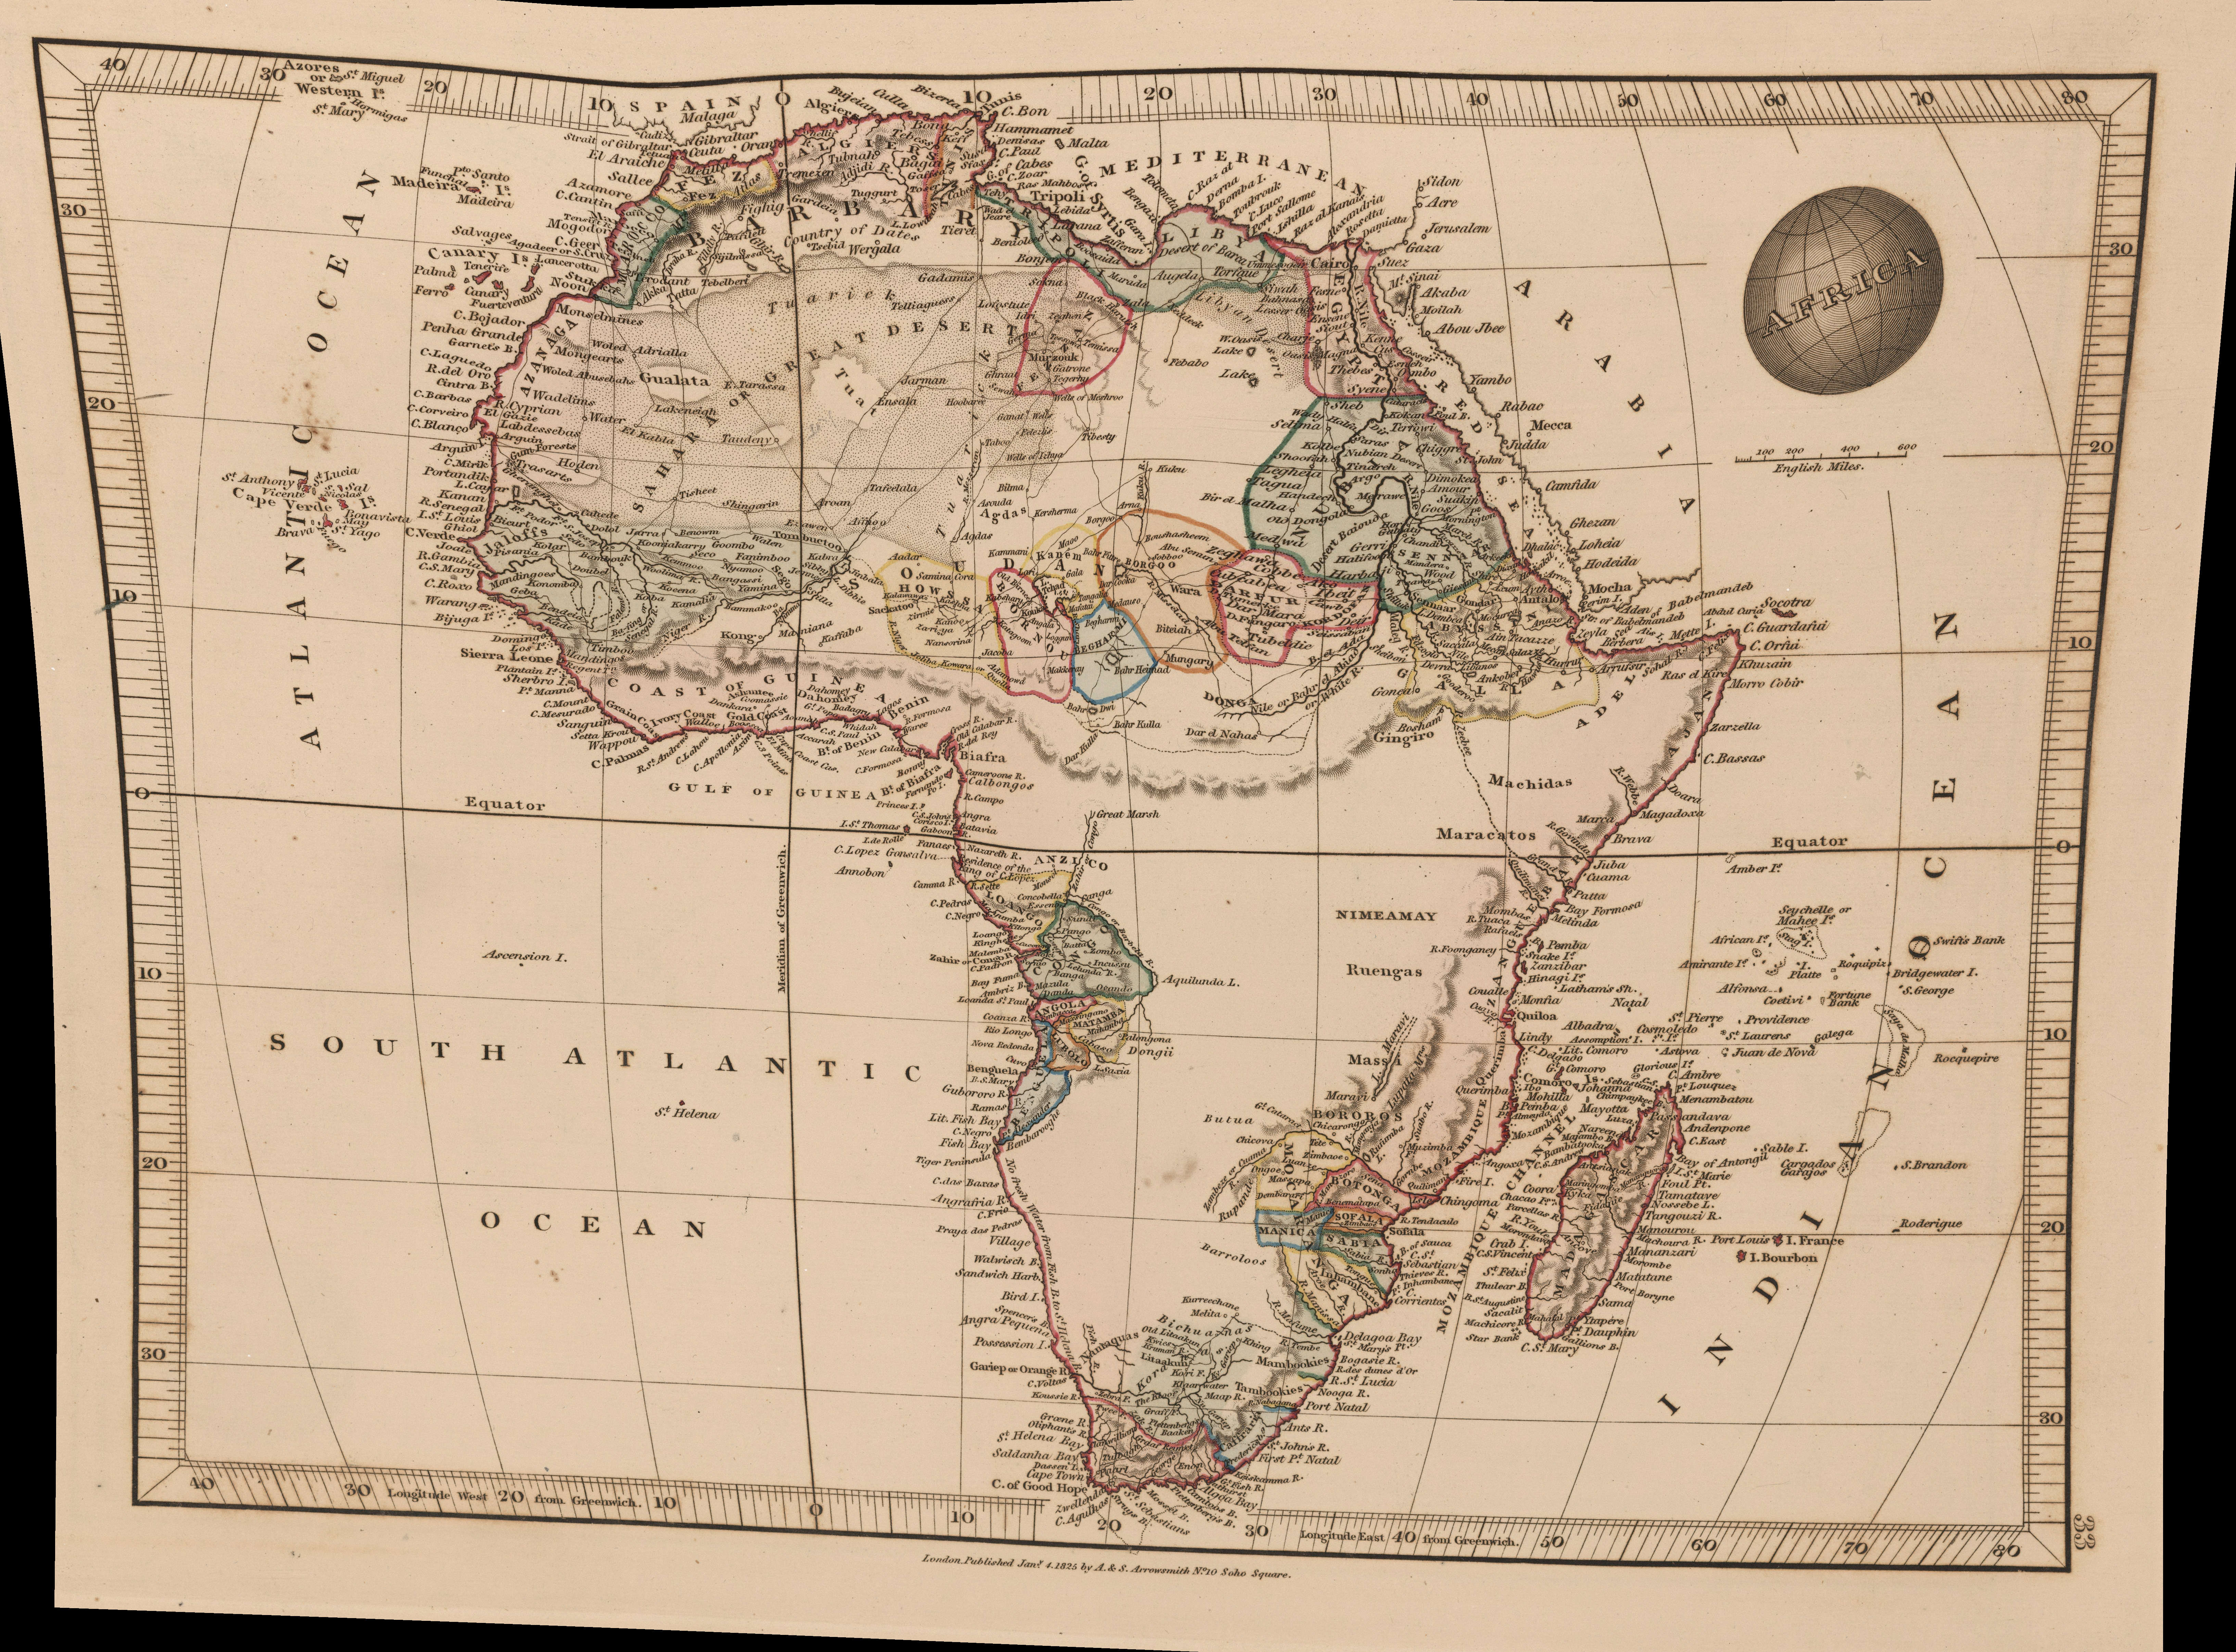
\includegraphics[width=\linewidth]{../img/Arrowsmith.jpg}
	\caption{Example of georeferenced map}%
	\label{Arrowsmith}
\end{figure}

%\begin{multicols}{2}

The accuracy of the historical maps used to create the polygons of the Geo-ISD
is a natural concern. Who typically drew these maps? Based on what sources? For
what purposes? And with what level of technical accuracy? 

Most of the maps from the David Rumsey project were from atlases published for
commercial purposes by individuals or small publishing companies specializing in
this type of publication. Most are from English or American atlases, but French,
Italian, German and other sources are included as well. The maps were based on a
combination of existing maps updated with `the latest sources' (a fact
frequently boasted in the title of the atlas), which for the majority of the
period meant explorers or geographers on missions from their respective
geographical societies.\footnote{Later maps additionally draw on the work of
military surveyors, but as far as I have been able to tell the majority are
still based primarily on the work of explorers and past maps.} In the words of
\citet[47-48]{Stone1995}: `Cartography in Africa [in the 19th century] is still
a mix of measurement, less accurate observations, word of mouth, previous maps
and sources, educated guesses and pure conjecture. Nevertheless a distinct
improvement on the maps of previous periods.' Because of this, I expect two
types of errors: errors resulting from measurement, that is technical or
cartographic errors, and bias resulting from misconceptions (deliberate or not)
of what constituted the borders of a polity at the time. I also expect errors to
be replicated by other maps, before eventually being corrected. One example of
this is the nonexistent Mountains of Kong, which can be seen in Figure
\ref{Arrowsmith} as the mountain range stretching across most of the continent
from East to West. These mountains were replicated for the better part of the
nineteenth century before eventually being wiped from the map
\citep{Bassett_1991}.

While the quote above might lead one to expect considerable cartographic error,
by my estimate this error amounts to 36.9km on average for the shapes included
in the GeoISD. This estimate is based on the estimated mean distance of the
coastline in the maps to the real coastline, along the borders of the states
that were traced. This captures cartographic error explicitly, because
regardless of where states did or did not extend their control, the coastline in
the map should line up with the real coastline. This means that there are often
multiple estimates for each map, reflecting how the accuracy is better in some
places than in others. If this difference was above 100km, the maps were deemed
too inaccurate and excluded from the sample. Error estimates were not made for
states that lay inland, because consistently matching features from the maps to
real geographical features was not feasible other than when using the coastline,
which provides a visible line of comparison. Additionally, such cartographic
error only adds noise, because there is no reason to suspect that the error
should be biased in any direction. It is just as likely to err toward the South
as it is to the North, or West etc. In other words, just as likely make
depictions of states smaller or larger. Thus it should not affect coefficient
estimates, but could potentially affect standard error estimates.


Although I have not been able to find sources discussing specifically how
cartographers determined the borders of different polities, it is probable that
they in large part relied on local verbal sources (word of mouth). An example of
this can be glimpsed in the exchange where the explorer Mungo Park effectively
dubbed the mountains of Kong.\footnote{`I gained the summit of a hill, from
	whence I had an extensive view of the country. Towards the south-east,
	appeared some very distant mountains, which I had formerly seen from an
	eminence near Marraboo, where the people informed me, that these
	mountains were situated in a large and powerful kingdom called Kong; the
	sovereign of which could raise a much greater army than the King of
Bambarra.' \citep[CHAPTER XVIII]{ParkMungo2011Titi}.} Alternatively, boundaries
were established when expeditions such as Park's were escorted by
representatives of the rulers of the various polities they passed through, until
reaching \textit{frontier towns}, where they would be met by representative of
the next ruler \citep{ParkMungo2011Titi}. In the maps resulting from such
encounters, both their sources as well as the cartographers themselves could
have introduced bias to the resulting maps. Sources were likely to be rulers or
their representatives, with incentives for aggrandisement. The explorers and
cartographers on their part represented European rulers with an eye toward
colonial expansion. It less clear how this would affect the resulting borders
drawn. One potential bias would be to exaggerate the domains of your own
governments prospective colonies, and vice versa. Another possibility is that
colonial cartographers under reported state sizes to declare `terra nullius'.
However, I did not observe any systematic differences between the maps based on
their nationality.\footnote{If drawing borders was driven by colonial ambitions,
there should be observable differences between the different colonial powers in
line with their differing colonial ambitions.} In fact, their colonial ambitions
could just as easily have promoted accuracy as any potential military
expedition would benefit from accurate information \citep{Bassett_1994}.

\subsection{A topographical representation of the state} 
\label{A topographical representation of the state}

At the very least there should be heterogeneity in the conceptualization of
territoriality. What determines where a given source (or the cartographer in the
second instance) draws the borders of a polity, or how this would vary with
their respective conceptualization of states, polities and ethnic groups, is
impossible do determine. However, thanks to (usually) having multiple maps for
each state, the variation can be leveraged to create a measure of the
\textit{degree} to which a state had a presence in a given area over the time
period as a whole. When maps disagreed on where the various borders were, I
interpret this as either true variation across time, or as an indication of the
ambiguity of where a given state had nominal or real control. In the areas where
all the maps agree, one could be quite sure that the given polity had real
presence.  While in areas where only one map indicated that the state was
present, this could either be wrong, an indication of nominal as opposed to more
real presence or some other form of limited presence. The coding process of
looking at hundreds of maps strengthened this initial intuition, and the
resulting figures of state presence drawn from the complete data lends it
further credence. Figure \ref{nigeria} demonstrates how the estimate of
pre-colonial state presence captures a topographical measure. The Northern
states of Sokoto (North-West), Borno (North-East) and Adamawa (East) are clearly
distinguishable, while the Southern states (primarily the Benin kingdom,
neighbouring Dahomey and the multiple Yoruba states) have a weaker presence and
blend more together. The reason for the lower state presence in the South is in
part that these kingdoms were younger or did not survive for as
long\footnote{some due to being colonised, others due to conflict with the
Sokoto Caliphate} as the Northern states. Potentially they conformed to fewer
mapmakers' and historians' conceptualisation of `state', as fewer sources
depicted them for the years that they were included in the ISD v2. Furthermore,
Figure \ref{nigeria} demonstrates how the presence of the Northern states
gradually fades away from the center. In some places it fades gradually, as the
Sokoto Caliphate to the South. This presumably reflects the temporary high water
mark of its southward expansion, before being repulsed by the Yoruba kingdom of
Ibadan as well as its less direct rule further from the core. In other places,
state presence fades rapidly, as Borno to the North, where its borders meet Lake
Chad.

%\end{multicols}

\begin{figure}[htpb]
	\centering
	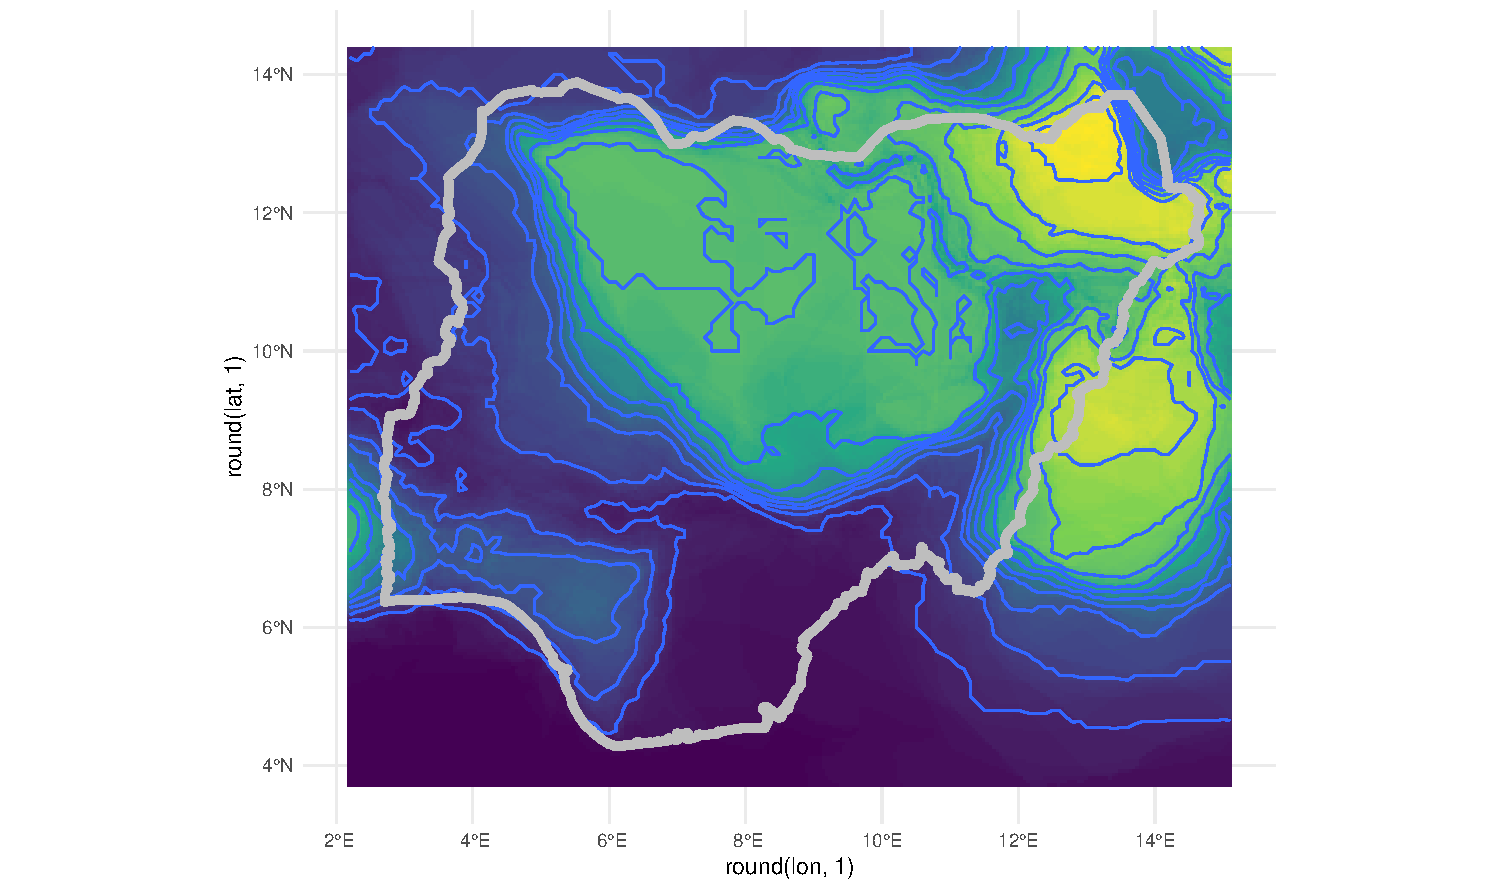
\includegraphics[width=\textwidth]{../../R/Output/nigeria.pdf}
	\caption{Pre-colonial state presence in Nigeria (1800-1914).}
	\label{nigeria}
\end{figure}

%\begin{multicols}{2}

The resulting data can be compiled in different ways, to provide different
insights. For the analysis in this paper I rely on a measure of `state
presence', similar in concept to that of `state history' introduced by
\citet{Depetris-Chauvin2016}.\footnote{The main difference between these
	measures is that `state history' is not a topographic measure, and
	usually only includes one shape per state, which implies static borders
	and uniform presence throughout the territory. It is also measured in 2
by 2 decimal degree grid cells, only includes Sub Saharan Africa, includes fewer
states despite going further back in time.} I measure `state presence' the as
number of state-shapes that indicate that a state was present in a cell. Thus
the interpretation is that if more maps indicate that a state was present in a
cell, it gets a higher state presence score, even when there are multiple
observations in a year. The benefit of this approach is more data and more
variation in the conceptualisations of statehood, which produces a more nuanced
and theoretically accurate measure of state presence. The downside is that it
increases the likelihood of bias on account of availability bias, whereby well
known states (from the mapmakers perspective) are overrepresented. I therefore
conducted robustness checks using a different version of the state presence
variable (see below). Both measures also take care to only count the state most
often present in each cell. If a cell contains 40 shapes of the Sokoto Caliphate
and 7 shapes of Borno, only the Sokoto shapes are counted. Including the Borno
shapes would risk over counting, as it most likely does not represent additional
state presence but rather overlapping or contested sovereignty. 

%\end{multicols}

\begin{figure}[htpb]
	\centering
	%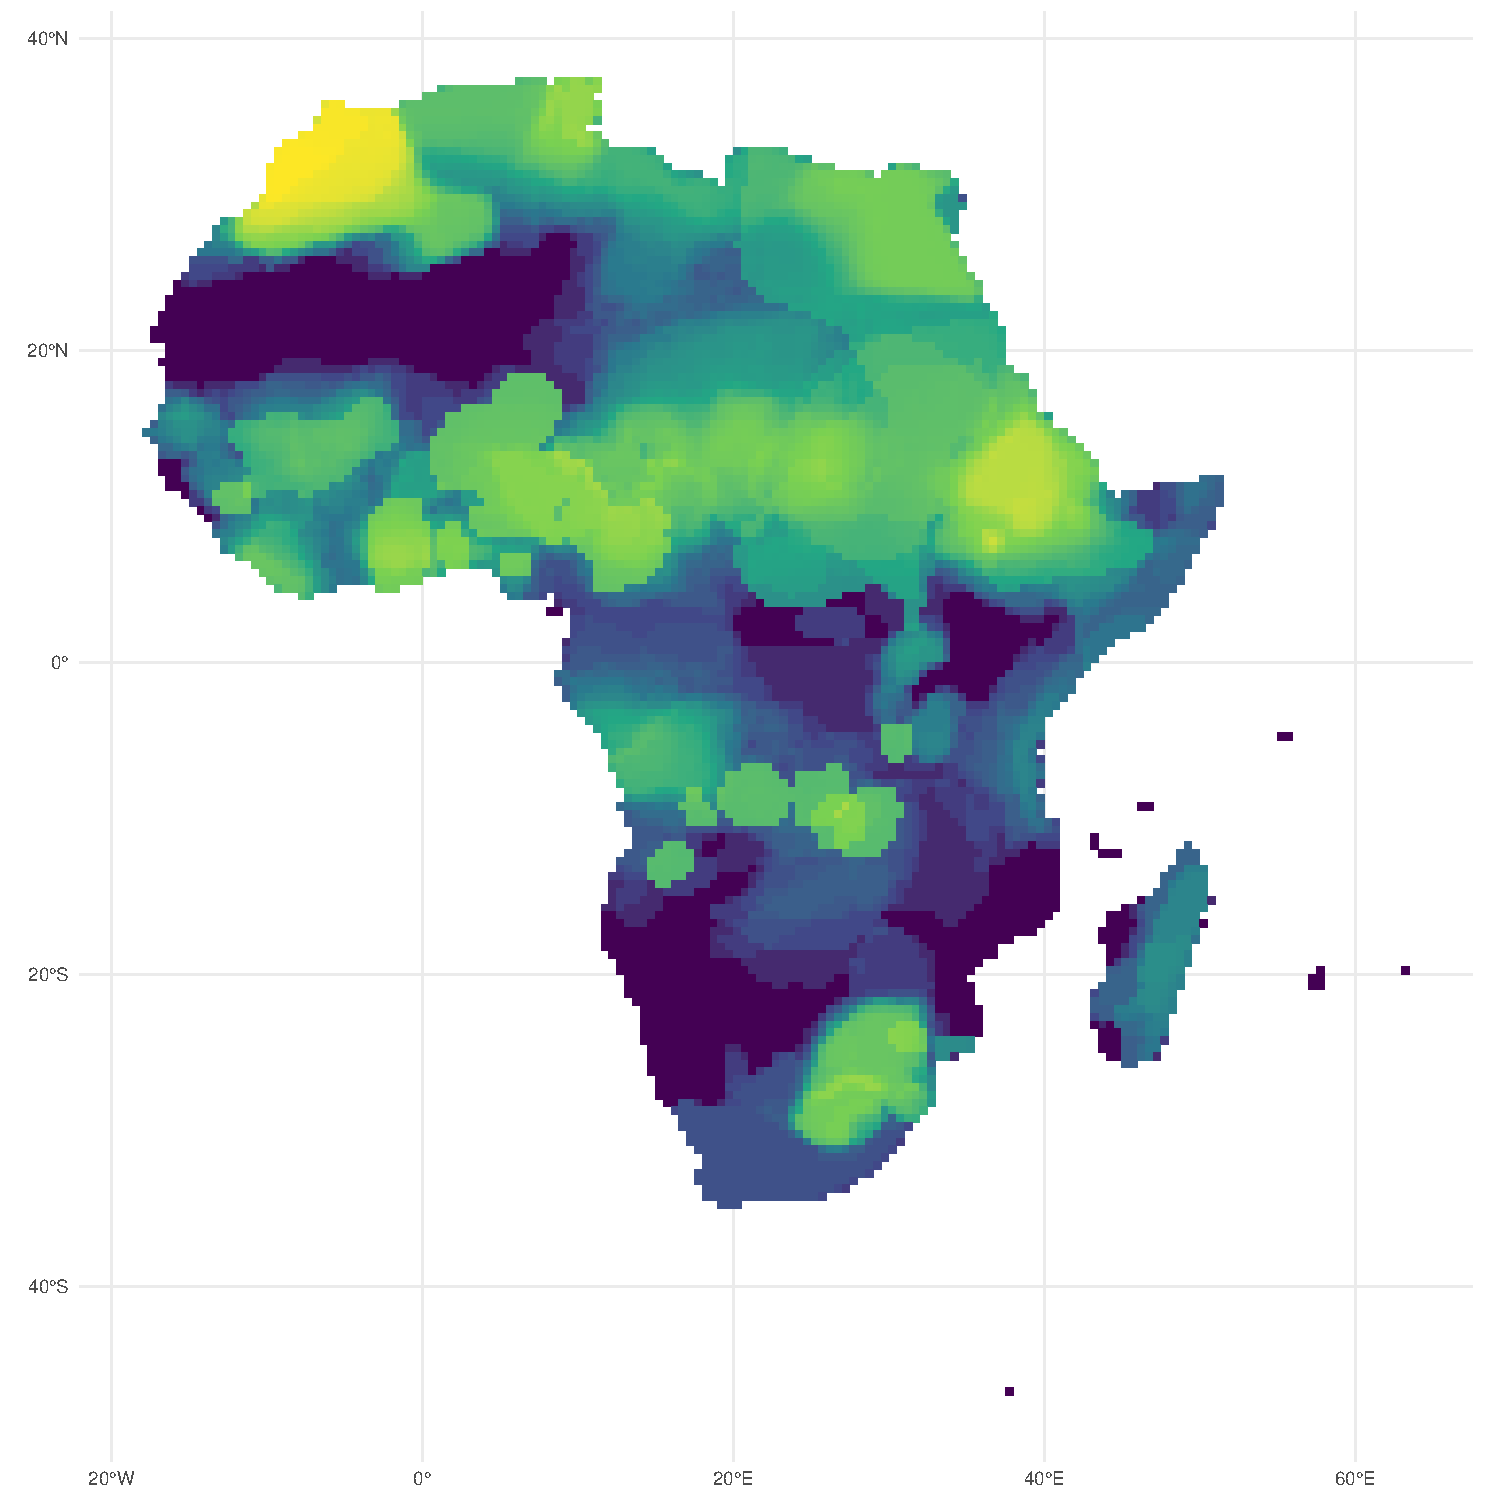
\includegraphics[width=0.8\linewidth]{../Rplot_ln_sp_int.pdf}
	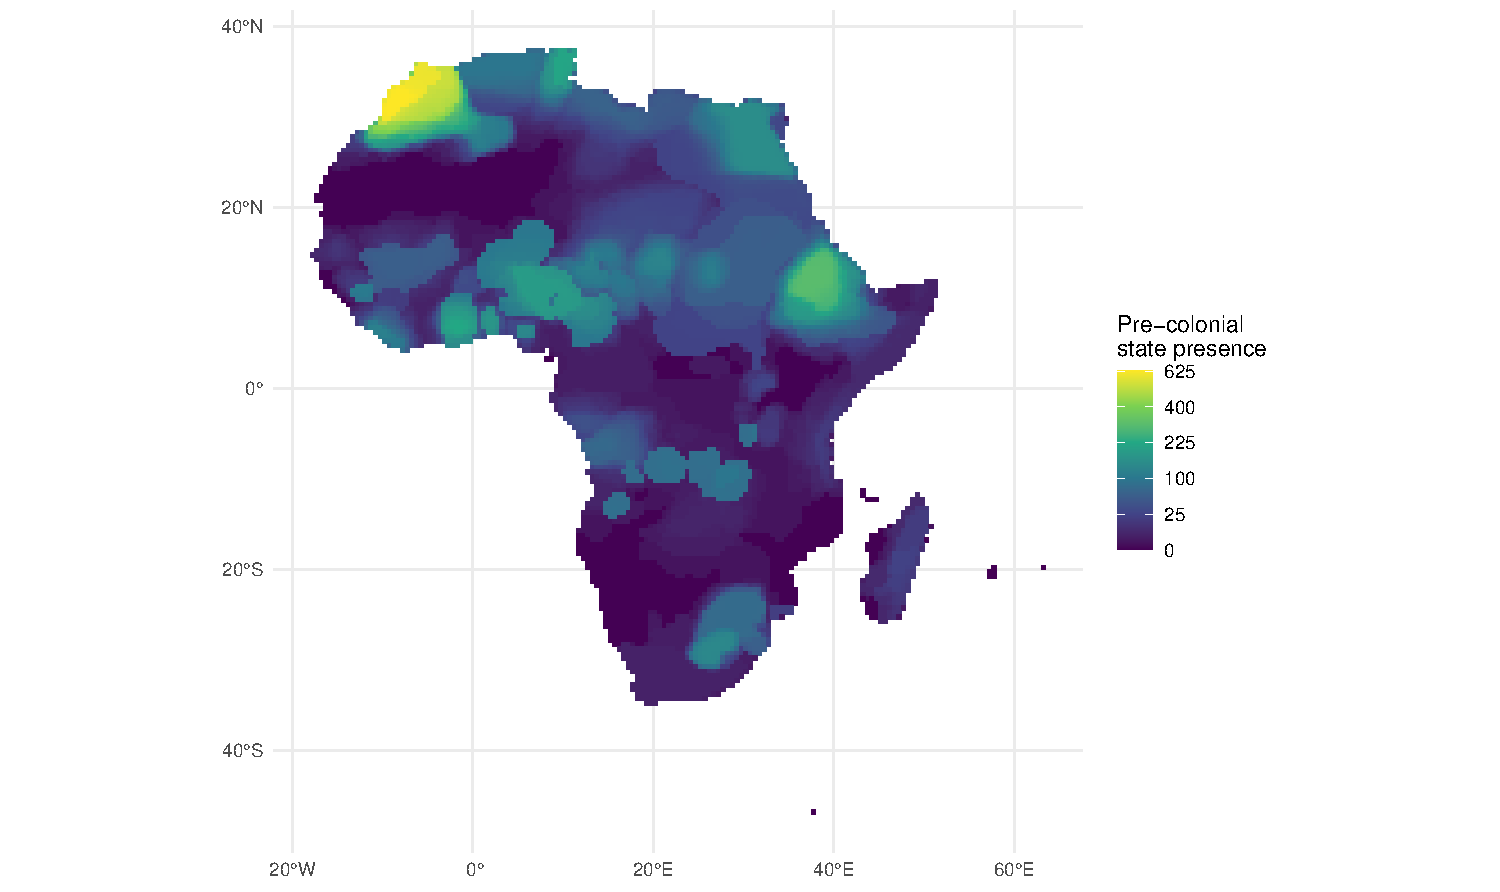
\includegraphics[width=\linewidth]{../../R/Output/spPlot.pdf} \caption{State presence (sqrt transformed) with interpolated years based on historical atlases.}
	\label{Sp_i}
\end{figure}

%\begin{multicols}{2}

Because I do not expect the relationship between pre-colonial state presence and
civil conflict to be linear and because the data are heavily skewed, the
variable is square root transformed. While log transformation is typically
employed in the literature, the variable contains zeros. This is usually solved
by adding a constant to all values. However, this could potentially introduce
bias, and complicates the interpretation of the results \citep{Ekwaru_2018}. I
therefore present the more conservative approach of using a square root
transformation for the main models.\footnote{In addition to the square root
	transformed version of the main independent variable, I also ran models
	using the more common log transformation. The results remained
substantially the same, but with larger effect sizes.} This has the benefit of
not having to add a constant but produces a less evenly distributed variable. 

In summary, the main explanatory variable is an interaction between pre-colonial
state presence (square root transformed) and distance to capital (log
transformed). The theoretical expectation is that pre-colonial state presence is
conflict reducing in areas close to the post independence capital and conflict
inducing in more remote areas. In other words the effect of pre-colonial state
presence is moderated by distance to the capital. Given how limited most
pre-colonial states were in size,\footnote{Due to limited technologies of state,
the late introduction of reliable guns and epizootics rendering travel on foot
the only option for large parts of the continent.} I expect positive effects of
pre-colonial state presence close to the capital to drop sharply. Consequently,
distance to the capital is log transformed anticipating a non-linear effect.
Because the variable is measured by distance from the center of each grid cell
to a point indicating the capital, there are no zeros and log transformation can
be done without adding a constant. Distance to capital is sourced from the
PRIO-grid data set but originally from \citet{Weidmann2010a}.

As a further robustness check I also ran models using a measure of state
presence that sums if there were any maps that included a state in a
grid-cell-year (as a sum of yearly dummies). In other words, this could be at
most 214 (one for each year in the sample period) and is more a measure of the
maximum \textit{extent} of state presence and less accurate in terms of
variations in depth. The benefit of this measure is that it avoids some of the
potential for over representation of countries frequently mapped by Europeans,
such as the North African states (due to proximity). As with the main measure of
state presence, only the shapes of the state that was most present in that grid
cell throughout the sample period were traced. Results remain substantially the
same for all specifications.

\subsection{Controls} \label{Controls}

The treatment variable predates the outcome by a long
period of time and there is a substantial risk of introducing post treatment bias
when including control variables. In choosing which control variables to
include, I balanced a trade off between potential post treatment bias
and omitted variable bias. 

Mountains facilitate early state formation by providing protection and limiting the
exit options of sedentary farmers \citep{Carneiro1988}. Mountainous terrain has
also been linked with civil conflict by providing shelter for rebel groups
\citep{Hegre2006}, although this relationship is debated \citep{Buhaug2002}. The
data is from the PRIO-grid data set, but originally from \citet{Blyth2002}, and
measures the percentage of the cell with mountainous terrain based on elevation,
slope and local elevation range.

Water is essential for state formation. States typically formed either around
coastal cities, close to navigable rivers or by the shores of great lakes.
People still tend to live next to a source of water. Proximity to water also acts
as a proxy for population density and fighting usually happens where there are
(at least some) people. The data on water as a percentage of the grid surface is
from the PRIO-grid data set but originally from the European Space Agency
\citep{Bontemps2009}. Because there are few only-water tiles (Lake Victoria
contains some exceptions), high levels primarily represent cells on the coast,
on the shores of great lakes or in a few cases the banks of great rivers.

Distance to the coast could affect both state presence and conflict in a number
of ways. First, as stated above, states were more likely form along the coast as
it connected cities and people. A special case for Africa is also the existence
of slave raiding/trading states that formed along the eastern and western coasts
of the continent. These states's raison d'être was raiding slaves from tribes and
peoples inland and selling them to coastal traders (European in the West and
Arab in the east). \citet{Nunn2008} argues that this left legacies of mistrust
and antagonism, which has resulted in increased levels of current day conflict.
Distance to the coast could also be related to the measure of state presence
through the fact that the measure is based on European observations (maps),
which had better coverage along the coast, especially for the earlier periods.
Distance to the coast could further be related to conflict through lower levels
of economic development inland. The distance to coast data is from
\citet{Wessel1996}. The variable was log transformed to account for a non-linear
relationship.

As with water, barren terrain could be a (negative) pre-condition for state
building as well as proxy for later population densities and thus could
correlate with both state presence and levels of conflict. The data are from
\citet{Bontemps2009}.

The states of North Africa are overrepresented in the Geo-ISD data due to the
geographical proximity and accompanying historical familiarity to European map
makers. This affects Morocco most particularly, as can be seen in Figure
\ref{Sp_i}, largely because the remaining North African states were under
Ottoman suzerainty for much of the period (and thus excluded from the data for
those years). If North Africa is also more or less conflict prone than the rest
of Africa on average, the inflated values of state presence would bias the
estimated coefficients. Accordingly, I included a dummy variable for the region
of North Africa.

Population density is added due to the theoretical expectation that it could be
a confounding variable. As discussed above, population density predicts both
state presence (states need a certain level of population density to form, and
survive \citep{scott2017against}), and conflict (conflict happens where there
are people). There are few accurate measures of population densities that
predate most of the states in the Geo-ISD that would avoid post treatment bias. The
best available estimates come from the HYDE project \citep{Goldewijk2016}, and I
use the estimates from 1600 as these pre-date most of the states in the Geo-ISD.
Despite its importance as a likely confounding variable, I only add population
density controls in the third step because there could still be post-treatment
bias arising from higher population densities from earlier state building projects.
Additionally, the HYDE data is partially based on backward extrapolation which
also might introduce post-treatment bias.

Distance to international boundaries could be related to state presence because,
despite their reputation, African borders were not drawn completely at random
(or along meridian lines). For example, the boundary between northern Nigeria and
Niger was based on the extent of the Sokoto Caliphate and the neighboring
Kanem-Bornu (or just Bornu) empire \citep{HiribarrenVincent2017AHoB}. Proximity
to an international boundary has also been found to predict conflict
\citep{Buhaug2002}. I use the measure included in the PRIO grid data, which is
originally from \citet{Weidmann2010a}.

\subsection{Modelling} \label{Modelling}

To minimize the impact of potential post treatment bias (vis-a-vis potential
omitted variable bias), controls were added step wise with increasing potential
for post treatment bias. The baseline model only includes geographic variables,
which should safely pre-date any states and thus be free of post-treatment bias.
Subsequent models add controls according to likelihood of introducing post
treatment bias.

To account for the dependent variable being count data (counts of deaths
(fatalities) and counts of conflict events), all model specifications reported
below are negative binomial regressions or zero inflated negative binomial
regressions. Likelihood ratio tests determined that negative binomial regression
provided a significantly better fit than Poisson regression.

The dependent variable contains excess zeros (8937 zeros relative to 100 counts
of 1 fatality, the second most frequent outcome). Additionally, the main
independent variable might affect the likelihood of any fatalities in a cell (or
if it remains a zero) differently to how it might influence the severity of
conflict once a cell has seen at least one fatality. I therefore use a zero
inflated negative binomial model. The first step of this two step approach is a
logit that models the likelihood that a cell is zero, in other words, that it
experiences no conflict. I used the same set of controls as I do not expect any
of them to exclusively affect conflict severity, nor do I expect their relation
to the main independent variable to be substantially different for an onset
model. The second step is a negative binomial estimation of conflict severity,
or the number of fatalities/events in a cell that has seen at least one
fatality/event.

Given what is known about spatial diffusion of conflict, there is reason to
suspect some spatial autocorrelation. However, controlling for this would
introduce a source of post treatment bias. Nevertheless, as an additional
robustness check I ran models with queen pattern spatial lags (Tables
\ref{spatialCount} and \ref{spatialZero}). The main results hold, albeit at the
10 percent significance level for the fatalities model.

\section{Results} \label{Results}

Despite the data on conflict starting nearly three decades after most of Africa
achieved independence (at which point the effects of pre-colonial state presence
on conflict should be most pronounced), there is a considerable conflict
inducing effect of high state presence far from the capital (see Table
\ref{interaction_interdeaths}). While the effect is only significant at the 10\%
level, the effect size is considerable (see Figure \ref{interdeaths} for
predictions based on the most inclusive model in Table A.2, which includes
controls for geography, North Africa, population density and distance to nearest
international border). Far from the capital, for an average amount of
pre-colonial state presence the model predicts 700 fatalities, as compared to
278 in remote cells with no pre-colonial state presence, and 4409 in cells with
high levels (225). While there is a significant negative effect of pre-colonial
state presence in the first two models, supporting H\textsubscript{1}, this
effect becomes insignificant after controlling for population density. Distance
to capital (log-transformed) is not significant in any of the models.
Surprisingly the distance to coast (log-transformed) is significant and
negative, even after controlling for population density. The rest of the
controls are either insignificant or behave as expected.

As discussed in Section \ref{Research design}, the data on fatalities contain
excess zeros, and a zero inflation model is probably a more correct
specification. Figure \ref{deaths_zinb} models the predictions of the first
second stage ZINB model included in Table \ref{zinbc}, which predicts the number
of fatalities in grid cells with at least one fatality. Taken together with the
negative binomial interaction (in Figure \ref{interdeaths}), it appears that
little-to-no pre-colonial state presence in the capital does not, by itself lead
to more fatalities in that area. However, if conflict does erupt in the capital,
states with some level of pre-colonial state presence appear far better at
quelling the violence. For capitals without pre-colonial state presence the
model predicts close to 20 000 fatalities, and an upper bound of over 58 000, as
compared to just under 2 300 with a mean level of pre-colonial state presence.
The effect size is even larger for the alternative state presence measure (see
`Alternative IV' in Tables \ref{robustc} and \ref{robustz}) with a predicted 48
152 additional fatalities in the capital grid cells with no pre-colonial state
presence (upper bound above 180 000). By comparison an average level of
pre-colonial state presence reduces the predicted fatalities (in the main ZINB
model) to just above 4 000 and just 207 for capitals with a high level of
pre-colonial state presence (225). These result suggest that local pre-colonial
experiences of statehood help states to contain outbursts of civil violence in
the capital, before events spiral out of control. Indeed, this is consistent
with the example of Burkina Faso, where the Mogho Naba of the Mossi kingdom of
Ouagadougou,\footnote{The royal title is only a ceremonial institution, but
wields considerable influence.} played a key role in brokering a deal that
allowed soldiers loyal to General Diendere to be peacefully confined in their
barracks following a failed coup, thus preventing further fighting between rival
sections of the armed forces in the capital. While 11 people died, and 271 were
wounded, the mediation by the traditional king is said to have prevented a
bloodbath \citep{Reuters2015, BBC2015}.

Although the effect sizes are less dramatic, the results for H\textsubscript{2}
hold for the ZINB models as well. For a mean level of pre-colonial state
presence, the model predicts almost 3 000 fatalities in grid cells far form the
capital, as compared to 1 853 for areas with no pre-colonial state presence and
7775 for remote areas with a high level of pre-colonial statehood (225).

The results for number of civil conflict events follow the same pattern as that
of fatalities for both negative binomial and ZINB models (see tables
\ref{interaction_both}, \ref{zinbc} \ref{zinbz}.

%\end{multicols}

\begin{figure}[htpb] \centering
	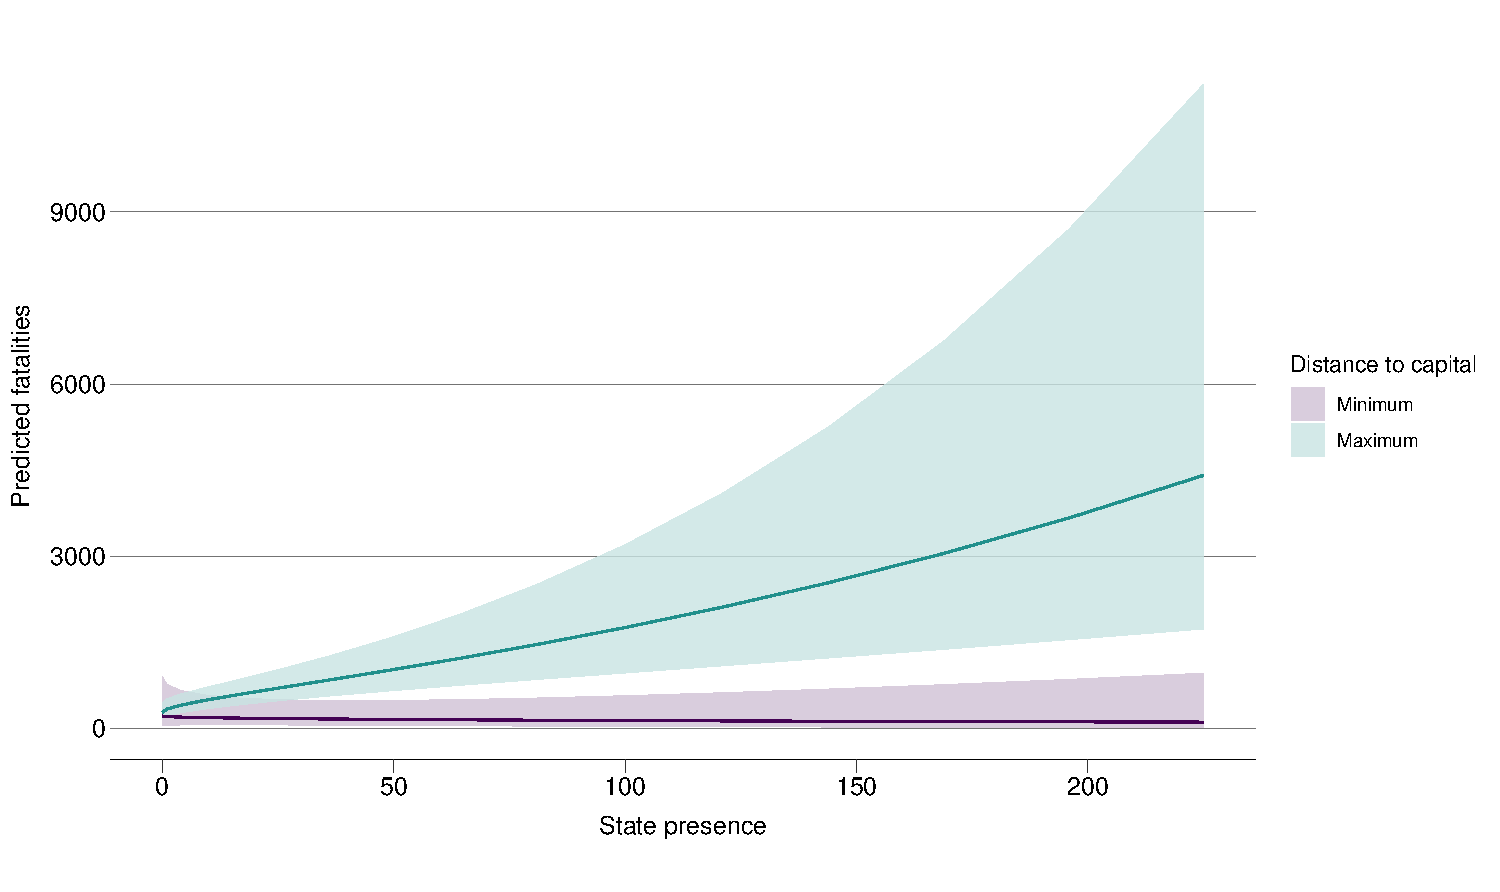
\includegraphics[width=\linewidth]{"../../R/Output/deathsInterPlot.pdf"}
	\caption{Marginal effect of pre-colonial state presence, conditioned on
	distance to capital.}
	\label{interdeaths}
\end{figure}

\begin{figure}[htpb]
	\centering
	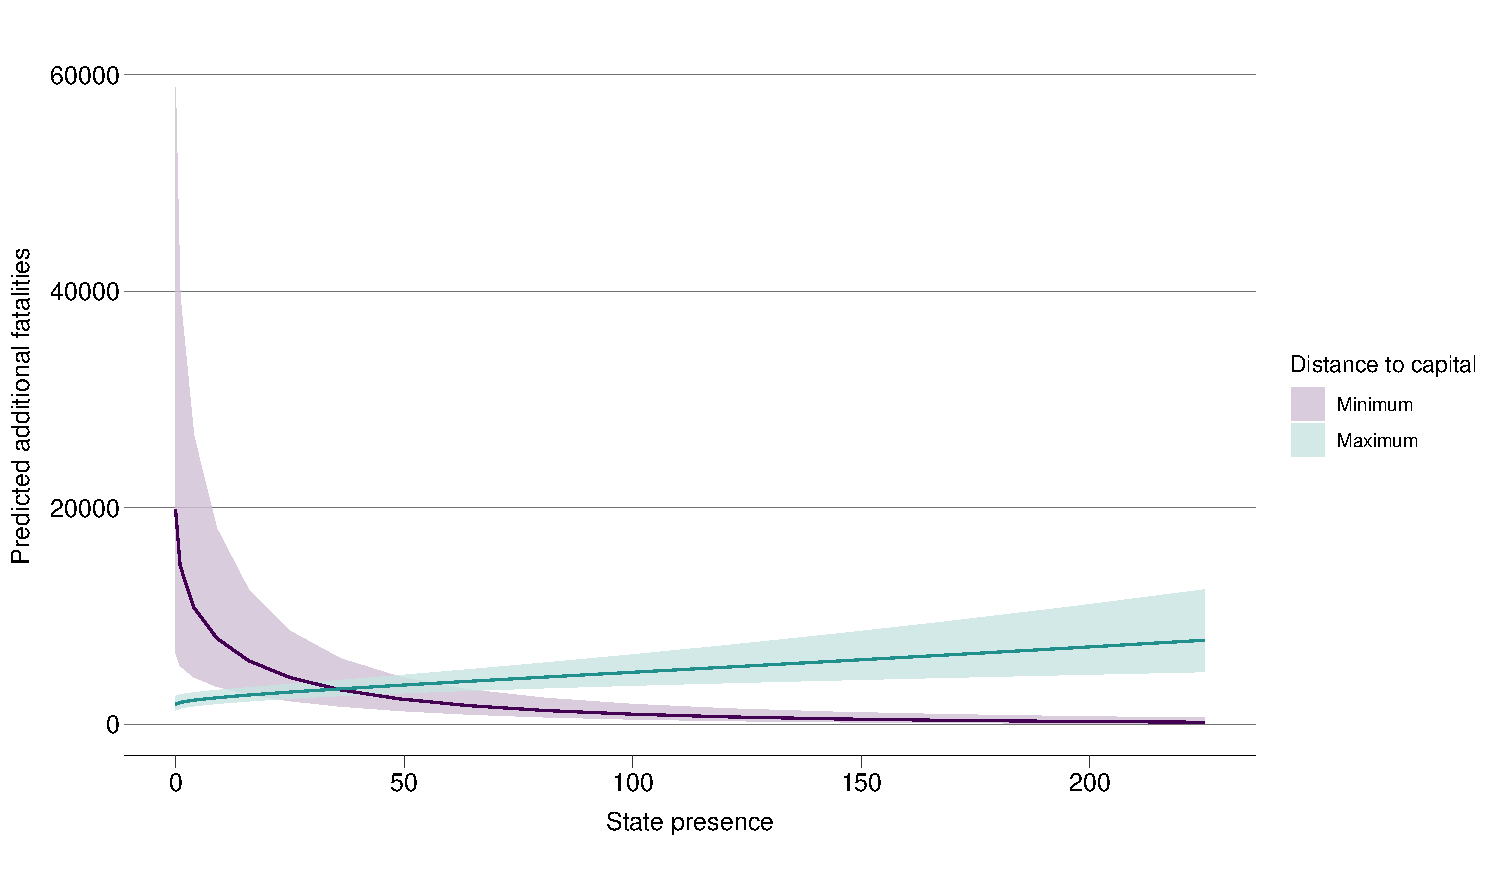
\includegraphics[width=\linewidth]{"../../R/Output/interdeathszinbplot.pdf"}
	\caption{Marginal effect of pre-colonial state presence, conditioned on
	distance to capital, in cells with at least one fatality (second stage
ZINB model).}
	\label{deaths_zinb}
\end{figure}

%\begin{multicols}{2}


\subsection{Alternative explanations} \label{Alternative explanations}

An alternative interpretation of the results could be that this is a story of
more coherent ethnic groups being more likely to be associated with states, and
more likely to (perhaps better able to) challenge the government when situated
far from the capital. However, getting closer to the real causality requires
untangling, for each case, if a given conflict is related to an ethnic group's
ties to a pre-colonial state or not. This lies outside the scope of this paper,
if it is even possible. Nevertheless, I ran models controlling the number of
excluded ethnic groups from the Ethnic Power Relations data per grid cell
\citep{Vogt2015} as an indication of whether the results are generally a story of
ethnic groups or not. The results from the main models hold albeit with a smaller
effect size (see tables \ref{robustc} and \ref{robustz}). This indicates (as
expected) that ethnic groups and exclusion matter, but that a significant effect
of pre-colonial state presence remains.

Another interpretation that is not controlled for in this paper is the
possibility that past conflict drives both state creation and current conflict.
However, data on past conflict is meager, especially so for Africa. To my
knowledge the \citet{Brecke1999} data set is the most complete. Even so, it
relies on written histories of which there is little for pre-colonial
sub-Saharan Africa. What is worse, the missing will be considerably biased
because kings and states are far more likely to chronicle their warfare in the
form of written records. What is more, there is good reason to believe that the
Tillyan notion that war made states, does not hold for Africa
\citep{Dincecco_2019}. 

Lastly, some have argued that differences in how different colonisers integrated
pre-colonial states have had an effect on whether or not institutions survived
the colonial era. Specifically that the British model of indirect rule tended to
preserve pre-colonial institutions, and that the French policy of direct rule at
least attempted to remove or supplant existing institutions \citep{Paine2019}.
However, how big the practical differences between the two approaches were,
given the same incentives for minimal administration, is debated
\citep{boone2014property, englebert2013inside}. If there was a real difference
and this coincided with differences in the likelihood that an area would be
colonized by the French or British (perhaps the British were more likely to
target areas they knew they could administer indirectly), it would represent a
confounding variable. Table \ref{robustc} and Table \ref{robustz} therefore
contain models running sub-samples excluding first former British and then
former French colonies. The results remain largely unchanged, albeit with
slightly smaller effect sizes when excluding former British colonies and
slightly larger when excluding former French. This is in line with the theory
suggesting that practices differed but whether this represents a significant
difference lies outside the focus of this article.

\section{Conclusion} \label{Conclusion}

Drawing on the emerging literature on pre-colonial states \citep{Paine2019,
Depetris-Chauvin2016}, institutions \citep{Wig2016, Englebert2002,
Michalopoulos2018} and civil conflict, and on newly compiled data, this paper
has re-examined the relationship between pre-colonial states and civil conflict.
I find support for both hypotheses. Overall, effect sizes are substantial,
indicating that levels of pre-colonial state presence have potentially had a
considerable impact on post cold war levels of civil conflict in Africa. While
armed conflict in capital areas is always a serious threat to the state, the
results in Tables \ref{zinbc} and \ref{zinbz}, and Figure \ref{deaths_zinb},
paint a far more dire picture in areas with little or no pre-colonial state
presence, perhaps reflecting state collapse. Pre-colonial state presence can be
conflict reducing, as suggested by some of the existing literature, but only by
providing states with a foundation for state building, which I argue made
capital areas more robust to civil conflict. On the other hand, in areas far
from the capital that have high levels of pre-colonial state presence, the
central state is not able to build on these existing institutions and source of
legitimacy. Instead, states struggle to integrate these areas without provoking
a violent response. The results are robust to alternative measurements of state
presence as well as conflict and to alternative model specifications.

An interesting case for the next decade is the relationship between Puntland and
Somalia. Puntland corresponds to the borders of the Majarteen sultanate and is
the only part of Somalia with strong pre-colonial state
presence.\footnote{Other parts have presence from Ethiopia and the Zanzibar
sultanate, and while three other Somali states are included in the ISD v2, only
Majarteen made into the GeoISD.} Following the break down of the central
Somali state, Majarteen (clan) leaders declared Puntland a autonomous federal
state over fears of the status of the Majarteen clan within post conflict
Somalia \citep{Johnson_2014}. The region has fared relatively well compared to the
rest of the country. While its leaders have cultivated continued ties to the
central government and aspirations of national leadership (as in the
post-independence period), they have also defended its autonomy. For example,
the local government has successfully resisted central state control over oil
prospecting in the northeast \citep{Johnson_2014}. As the central state in
Mogadishu grows more stable, it will call for regional reintegration. The
results presented in this paper suggest that such efforts might lead to yet more
violence in Somalia. Given that Puntland reportedly spends around 90\% of its
budget on security, police and recurrent administration \citep{Johnson_2014},
its leaders are signalling their intention of maintaining autonomy.

These findings have a few general implications as well. First, they demonstrate
that pre-colonial states can be a blessing or a curse depending on whether they
form the basis of the modern state or a point of opposition to it. Second, the
findings of this article demonstrate that local political histories matter, and
should be taken into consideration by policymakers and scholars alike. Finally,
these results lend credence to the general idea of the literature on artificial
states. However, more research using global data is needed to test whether
general trends for Africa hold outside that continent as well.

%\end{multicols}
\clearpage

\bibliographystyle{apsr}
\bibliography{../../lib.bib}

\label{lastpage}
\clearpage
\appendix

\section{Online Appendix: additional tables and figures}

% Setting tables and figures to count in the appendix
\setcounter{table}{0}
\renewcommand{\thetable}{A.\arabic{table}}

\setcounter{figure}{0}
\renewcommand{\thefigure}{A.\arabic{figure}}

\renewcommand{\thepage}{\arabic{apppage}}
\fancyfoot[C]{Page~\thepage~of~\pageref{applastpage}}
\pagenumbering{arabic}

\import{../../R/Output/}{atlasmaps.tex}

\import{../../R/Output/}{interaction_interdeaths.tex}
\import{../../R/Output/}{interaction_both.tex}
\import{../../R/Output/}{zinbc.tex}
\import{../../R/Output/}{zinbz.tex}

\import{../../R/Output/}{robust.tex}
\import{../../R/Output/}{robustz.tex}

\begin{figure}[htpb]
	\centering
	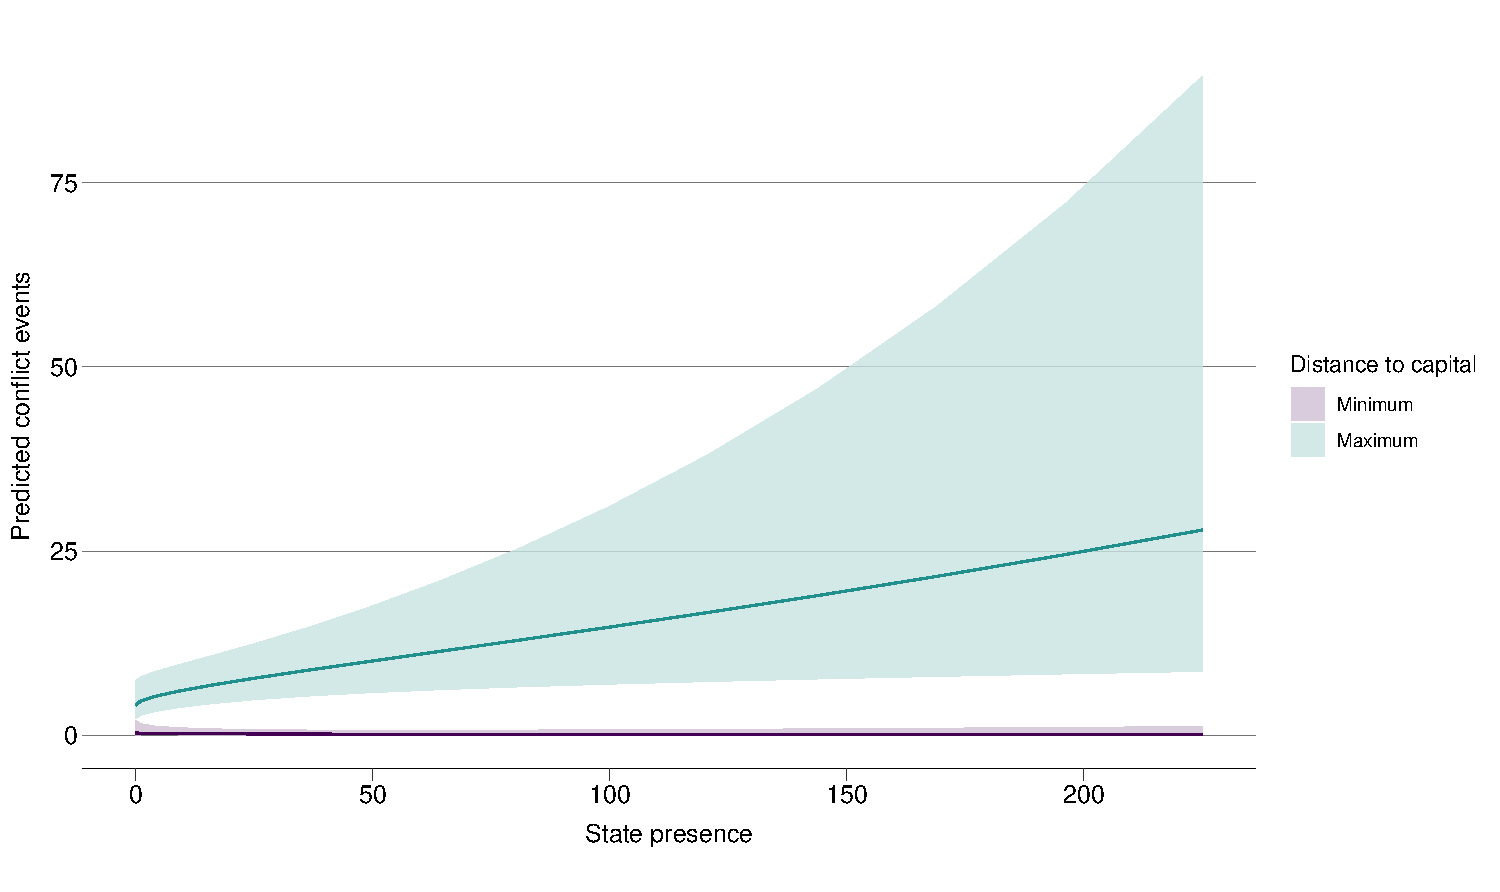
\includegraphics[width=\linewidth]{"../../R/Output/ggBothPlot.pdf"}
	\caption{Predicted conflict events per state presence, grouped by
	distance to capital.}
	\label{both_int}
\end{figure}

\begin{figure}[htpb]
	\centering
	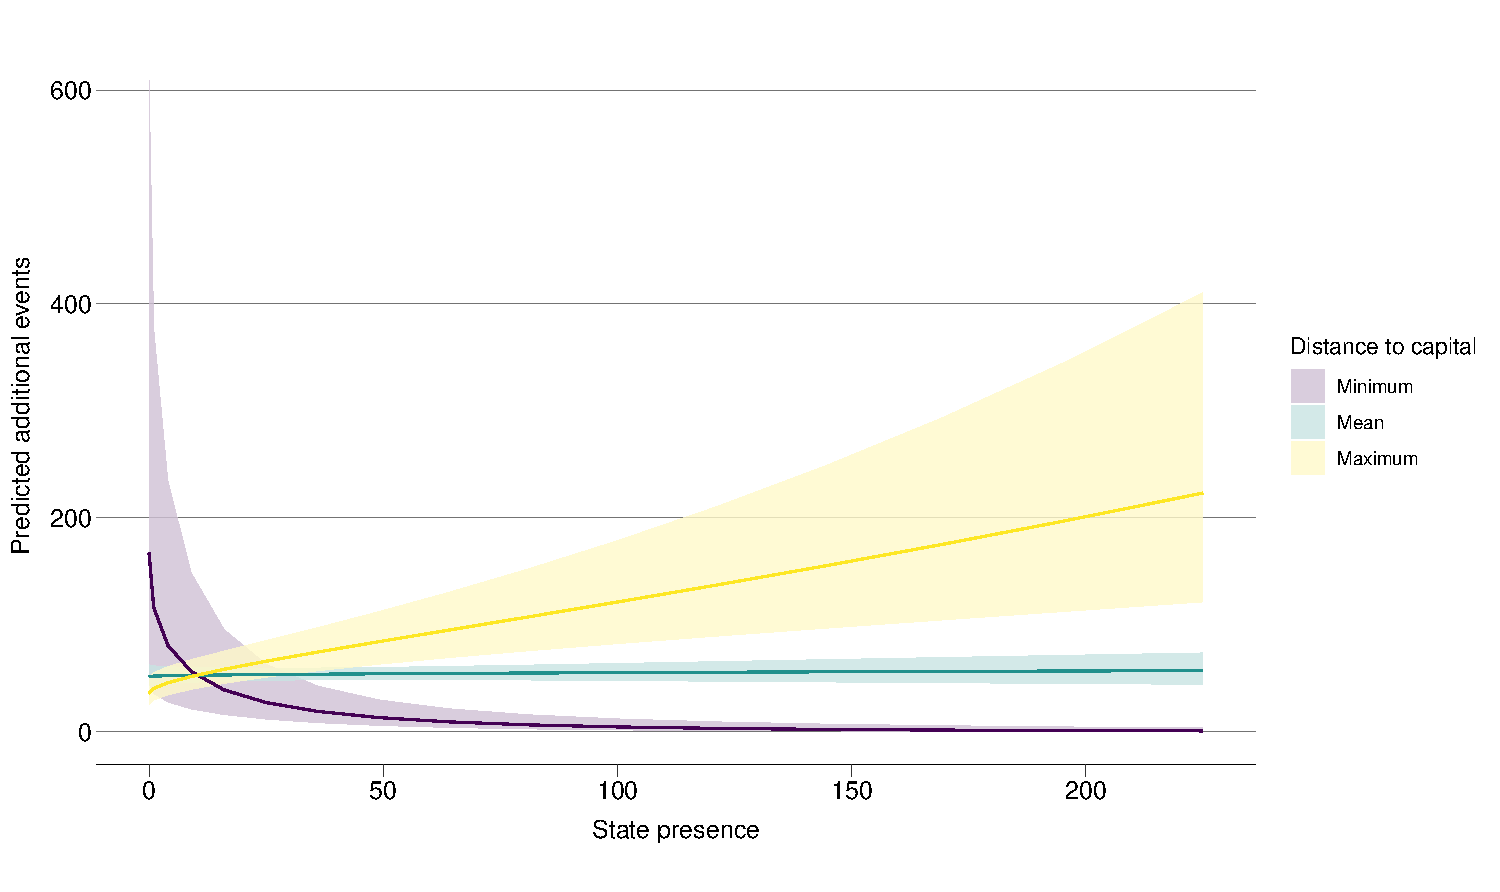
\includegraphics[width=\linewidth]{"../../R/Output/bothzinbplot.pdf"}
	\caption{Predicted conflict events per state presence, grouped by
	distance to capital, in cells with at least one conflict event.}
	\label{bothzinb_int}
\end{figure}

\begin{figure}[htpb]
	\centering
	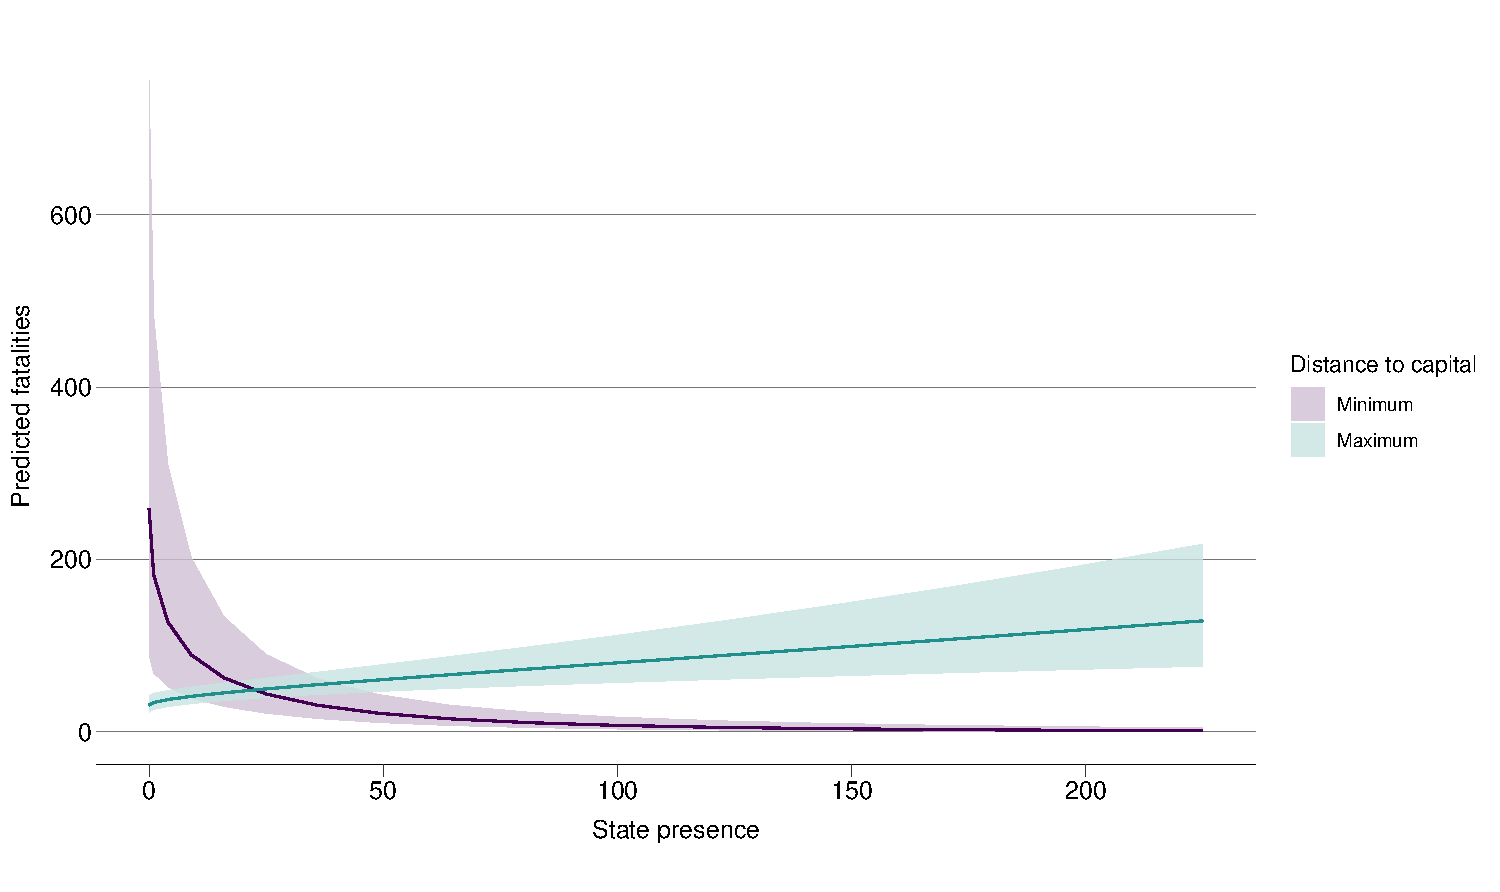
\includegraphics[width=\linewidth]{"../../R/Output/spatialzinbbothplot.pdf"}
	\caption{Predicted conflict events per state presence, grouped by
	distance to capital, in cells with at least one conflict event,
controlling for spatial diffusion.}
	\label{spatbothzinb_int}
\end{figure}

\import{../../R/Output/}{spatial_count.tex}
\import{../../R/Output/}{spatial_zero.tex}

\label{applastpage}

\end{document}
